%%%%%%%%%%%%
%
% $Autor: Theilmann $
% $Datum: 11.06.2024 $
% $Pfad: DemonstratorSchrittmotor\Assembly\Chapters\de\VorMontage.tex $
% $Version: 1 $
% !TeX spellcheck = en_GB/de_DE
% !TeX encoding = utf8
% !TeX root = MontageDemontageanleitung 
% !TeX TXS-program:bibliography = txs:///biber
%%%%%%%%%%%%

\chapter{Montage}\label{Mont}
In diesem Kapitel wird die Montage des Demonstrators für einen Schrittmotor Schritt für Schritt erläutert. Es wird empfohlen, die Schritte in der vorgegebenen Reihenfolge zu befolgen.


\section{Erster Schritt: Montieren Schaltnetzteil, Entwicklerboard und AMS1117}
 Montieren Sie die folgenden Bauteile und elektrischen Komponenten wie in Abbildung \ref{1.S} gezeigt. 
 
\begin{enumerate}
 	\item Befestigen Sie das Schaltnetzteil an der Bodenplatte mit 2 $\times$ $ M3 \times 10 \ mm $ Schrauben. Die Schrauben werden von der unteren Seite der Bodenplatte eingeführt. 
 	\item Nehmen Sie 2 $\times$ $ M3 \times 14 \ mm $ Schrauben und kontern Sie diese mit 2 $\times M3 $ Muttern gegen die Bodenplatte. Die Schrauben werden von der unteren Seite der Bodenplatte eingeführt.
 	\item Montieren Sie das Entwicklerboard Schrittmotorsteuerung A4988 auf der Bodenplatte. Verwenden Sie 2 $\times$ $ M3 \times 14 \ mm $ und 4 $\times$ $ M3 $ Muttern. Die Reihenfolge ist: Schraube - Bodenplatte - Mutter - Entwicklerboard - Mutter. Die Schrauben werden von der unteren Seite der Bodenplatte eingeführt.
 	\item Stecken Sie die Schrittmotorsteuerung in das Entwicklerboard und achten Sie auf die richtige Pinbelegung.
 	\item Setzen Sie den Spannungswandler AMS1117 in den Halter für AMS und setzen Sie den Clip auf. Befestigen Sie den Halter und den Clip mit einer  $\times$ $ M3 \times 14 \ mm $ Schraube
\end{enumerate}
 
\begin{figure}[H]
	\begin{center}
		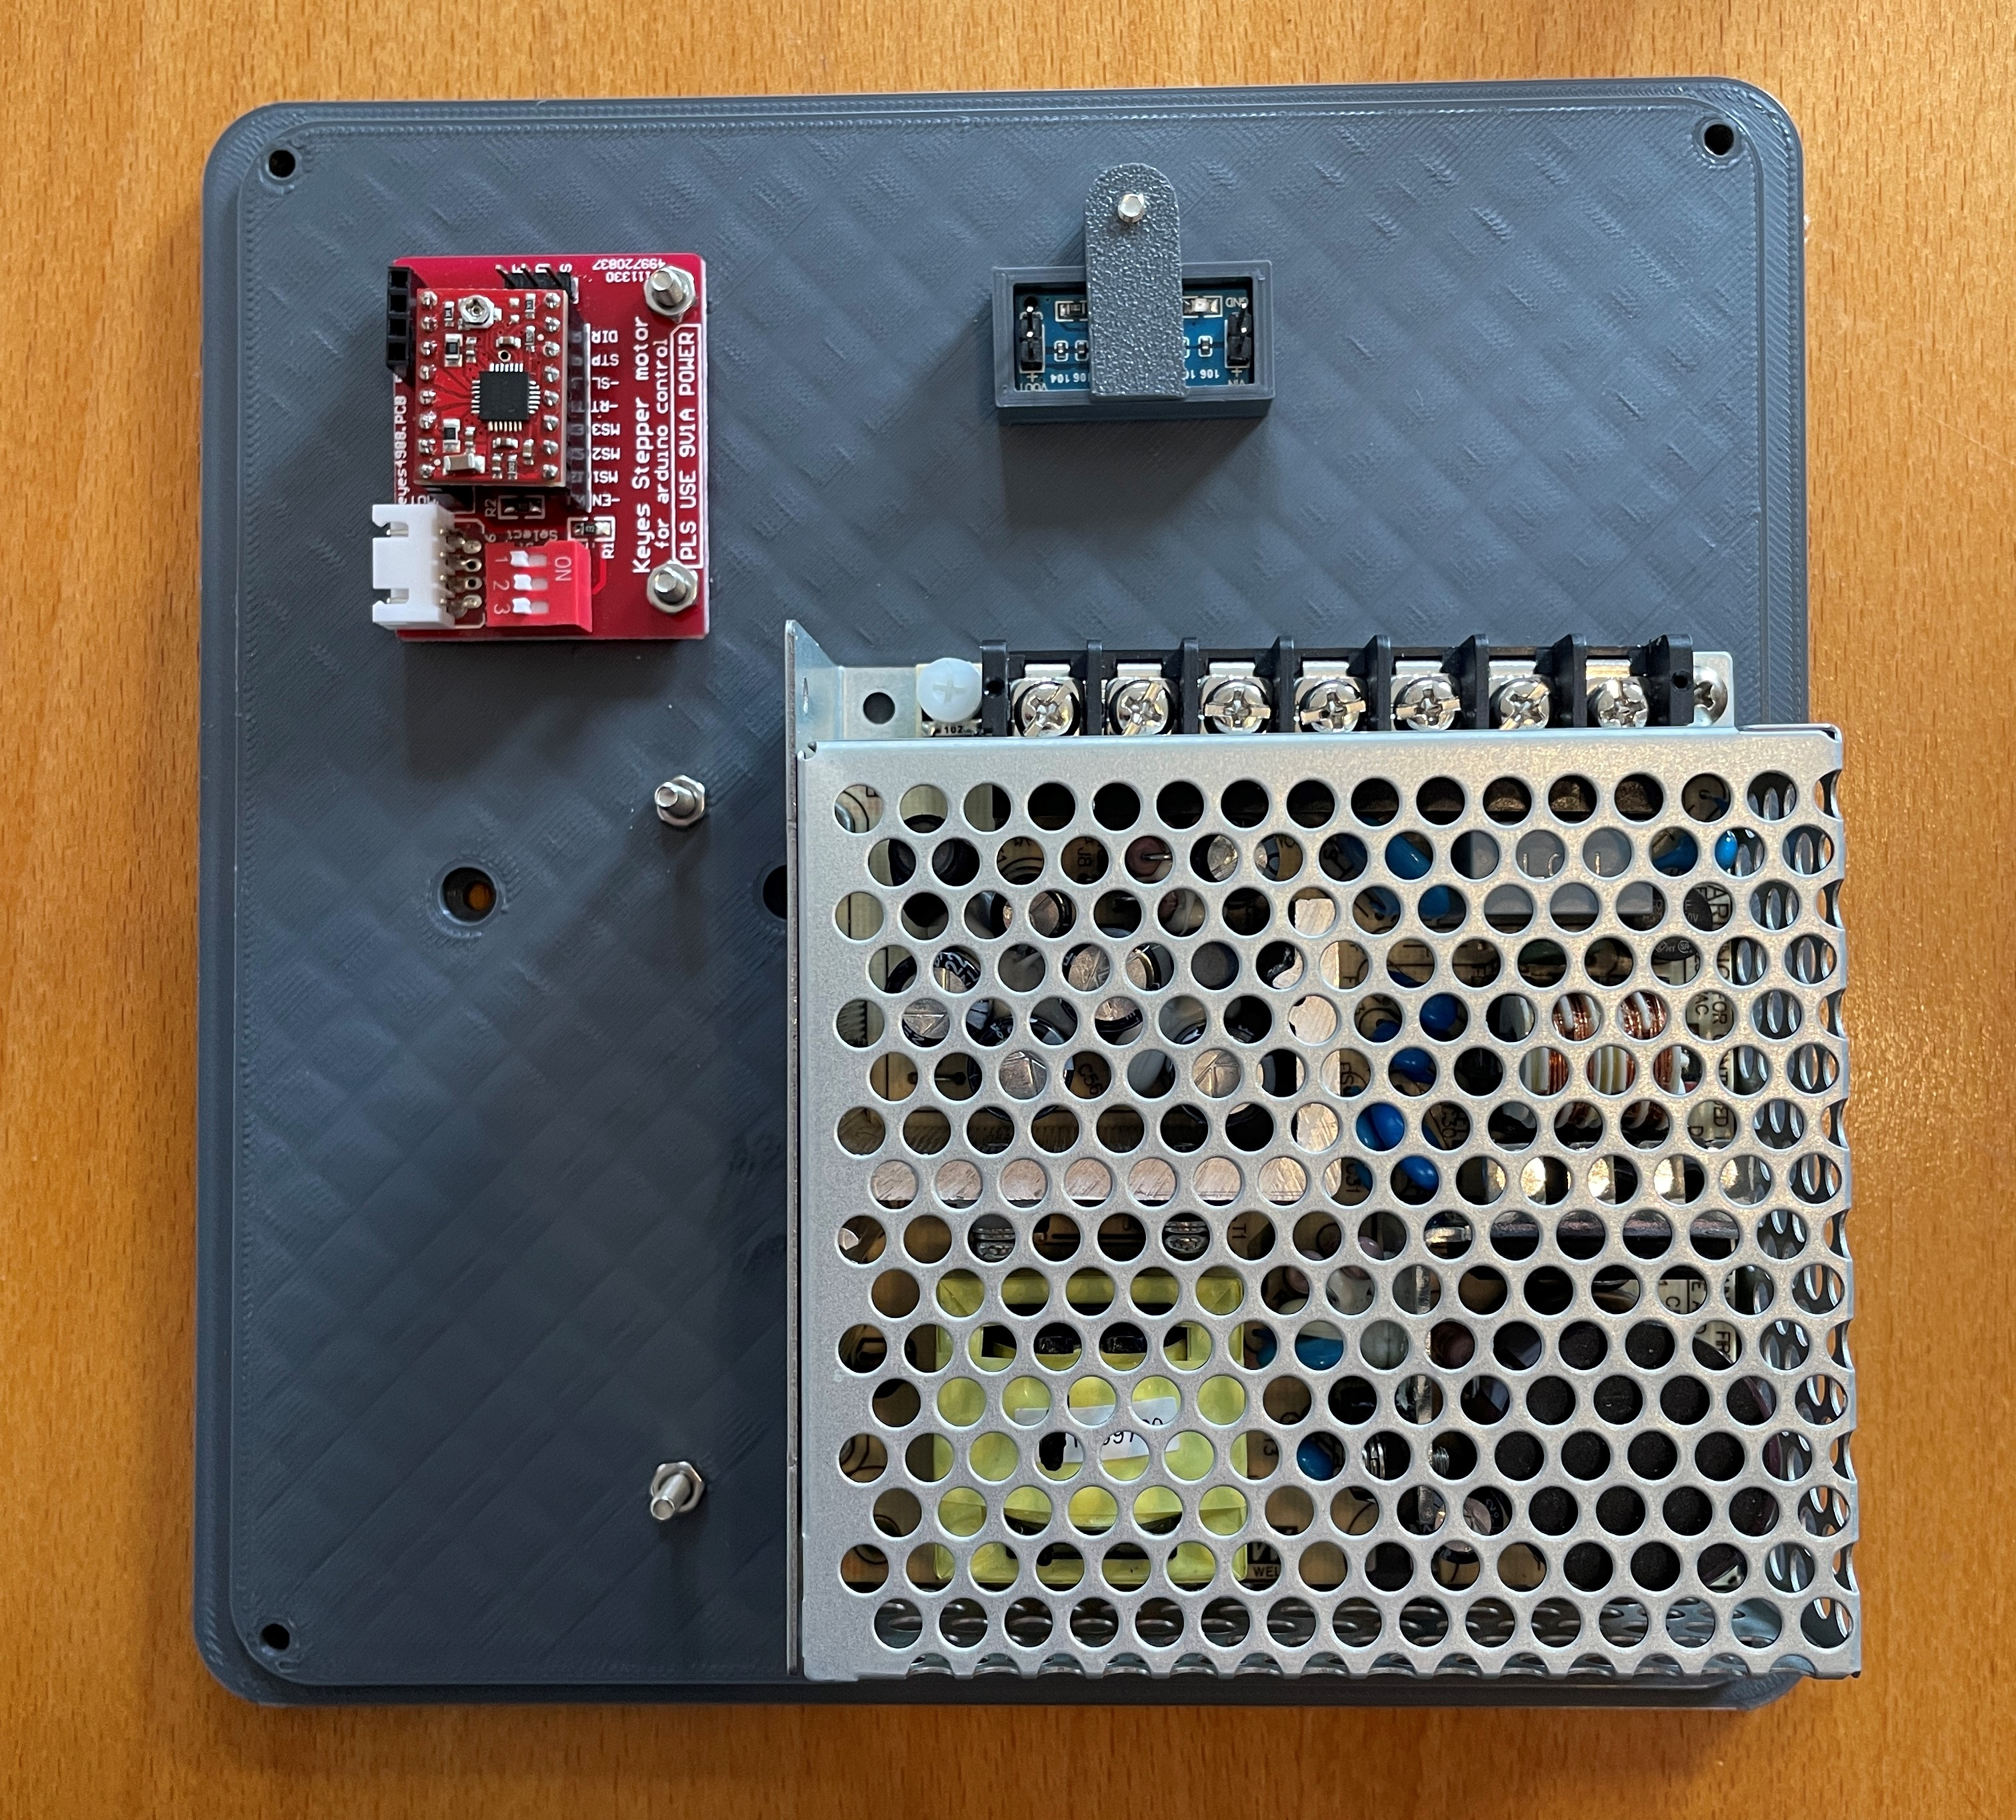
\includegraphics[width=\textwidth]{Images/1Schr.jpg}
		\caption{Erster Schritt: Montieren Schaltnetzteil, Entwicklerboard und AMS1117} \label{1.S}
	\end{center}
\end{figure}


\section{Zweiter Schritt: Anbringen der Bodenplatte an Aluprofil}
Montieren Sie die folgenden Bauteile und elektrischen Komponenten wie in Abbildung \ref{2.S} gezeigt.

\begin{enumerate}
	\item Führen Sie 2 $\times$ $ M3 $ Hammermutter in das Aluprofil ein.
	\item Verschrauben Sie die Bodenplatte mit 2 $\times$ $ M3 \times 10 \ mm $ Schrauben an den Hammermuttern im Aluprofil, sodass die Bodenplatte bündig mit dem Profil abschließt.
	\item Setzen Sie das Tiny Machine Learning Shield (TMLS) auf die hervorstehenden Schrauben und sichern Sie es mit 2 $\times$ $ M3 $ Muttern.
	Stecken Sie den Arduino Nano Sense BLE 33 Lite auf das TMLS und achten Sie dabei auf die Pinbelegung.
\end{enumerate}

\begin{figure}[H]
	\begin{center}
		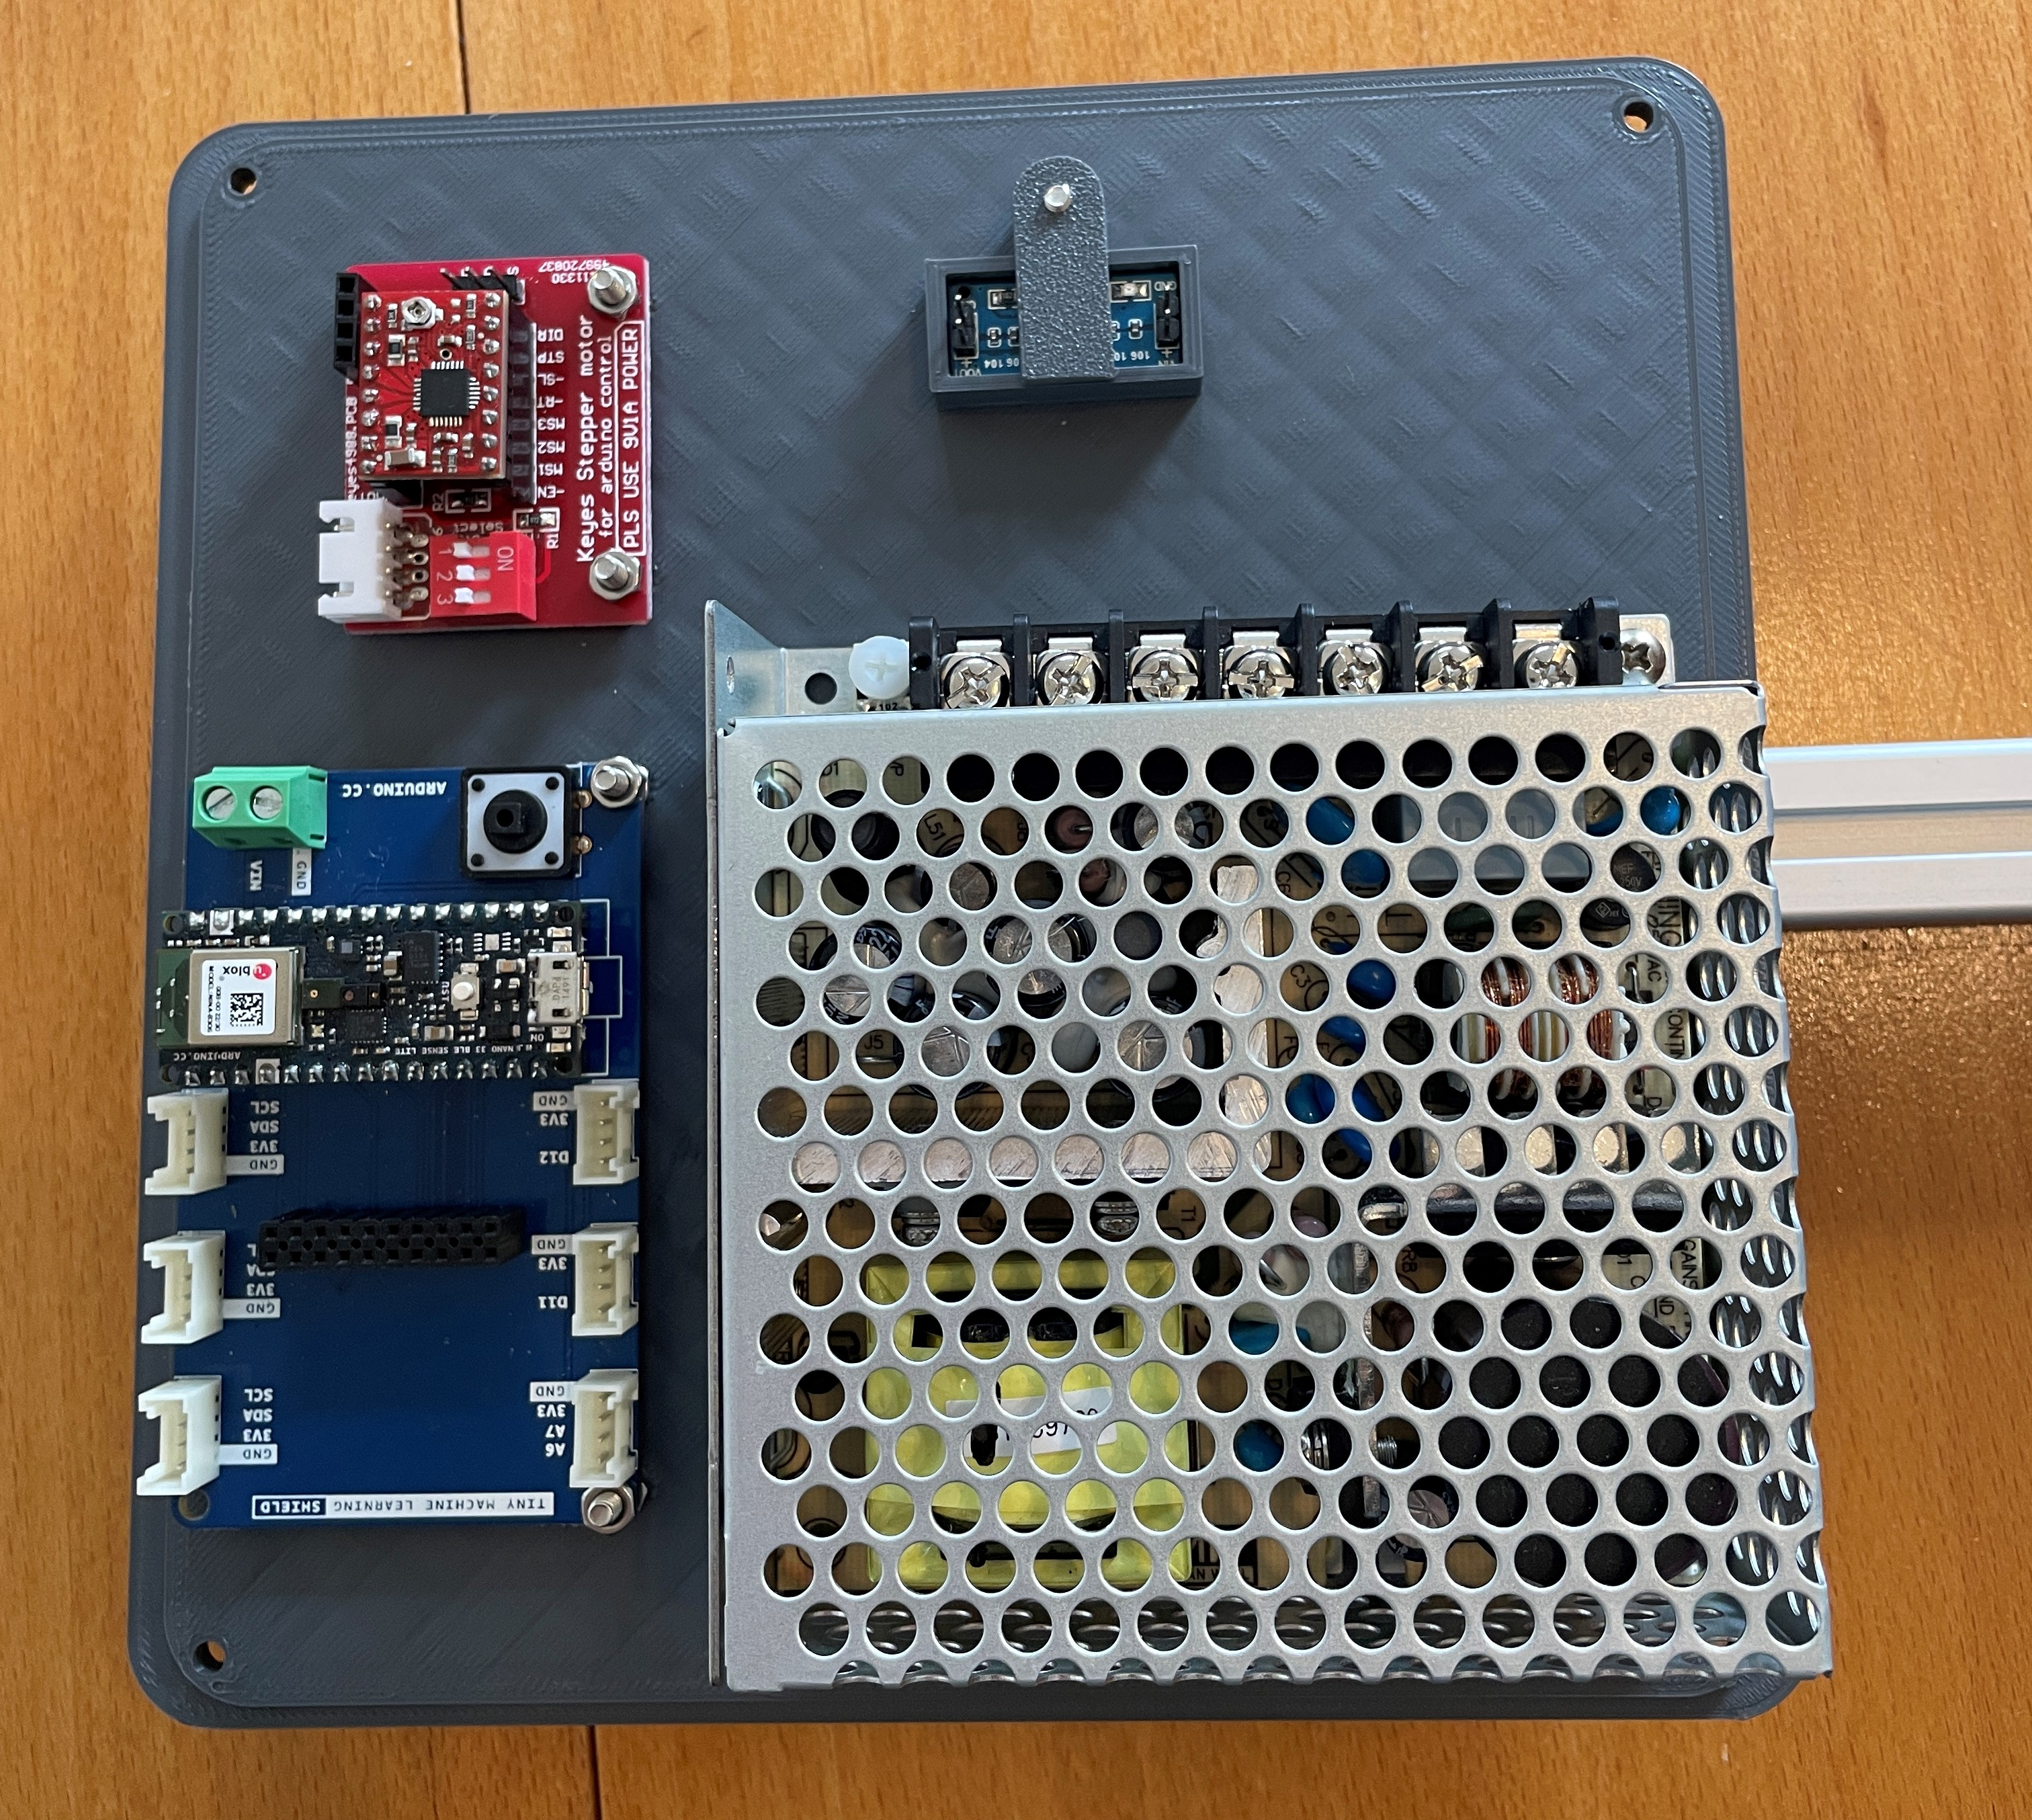
\includegraphics[width=\textwidth]{Images/2Schr.jpg}
		\caption{Zweiter Schritt: Anbringen der Bodenplatte an Aluprofil} \label{2.S}
	\end{center}
\end{figure}


\section{Dritter Schritt: Zusammenbau der Vorderplatte}
Montieren Sie die folgenden Bauteile und elektrischen Komponenten wie in Abbildung \ref{3.S} gezeigt.

\begin{enumerate}
	\item Befestigen Sie das OLED-Display mit 2 $\times$ $ M3 \times 6 \ mm $ Schrauben in die dafür vorgesehenen \O 2,8 \ mm Bohrungen der Vorderplatte.
	\item Führen Sie die SMD-LED in die \O 8 \ mm Bohrung der Vorderen Platte ein.
	\item Führen Sie den Drehwinkel-Encoder in die \O 7 \ mm Bohrung ein und kontern Sie diese mit der P-4 Mutter.
	\item Führen Sie den Druckknopf in die \O 13,5 \ mm Bohrung und kontern Sie den mit der zugehörigen Mutter.
\end{enumerate}

\begin{figure}[H]
	\begin{center}
		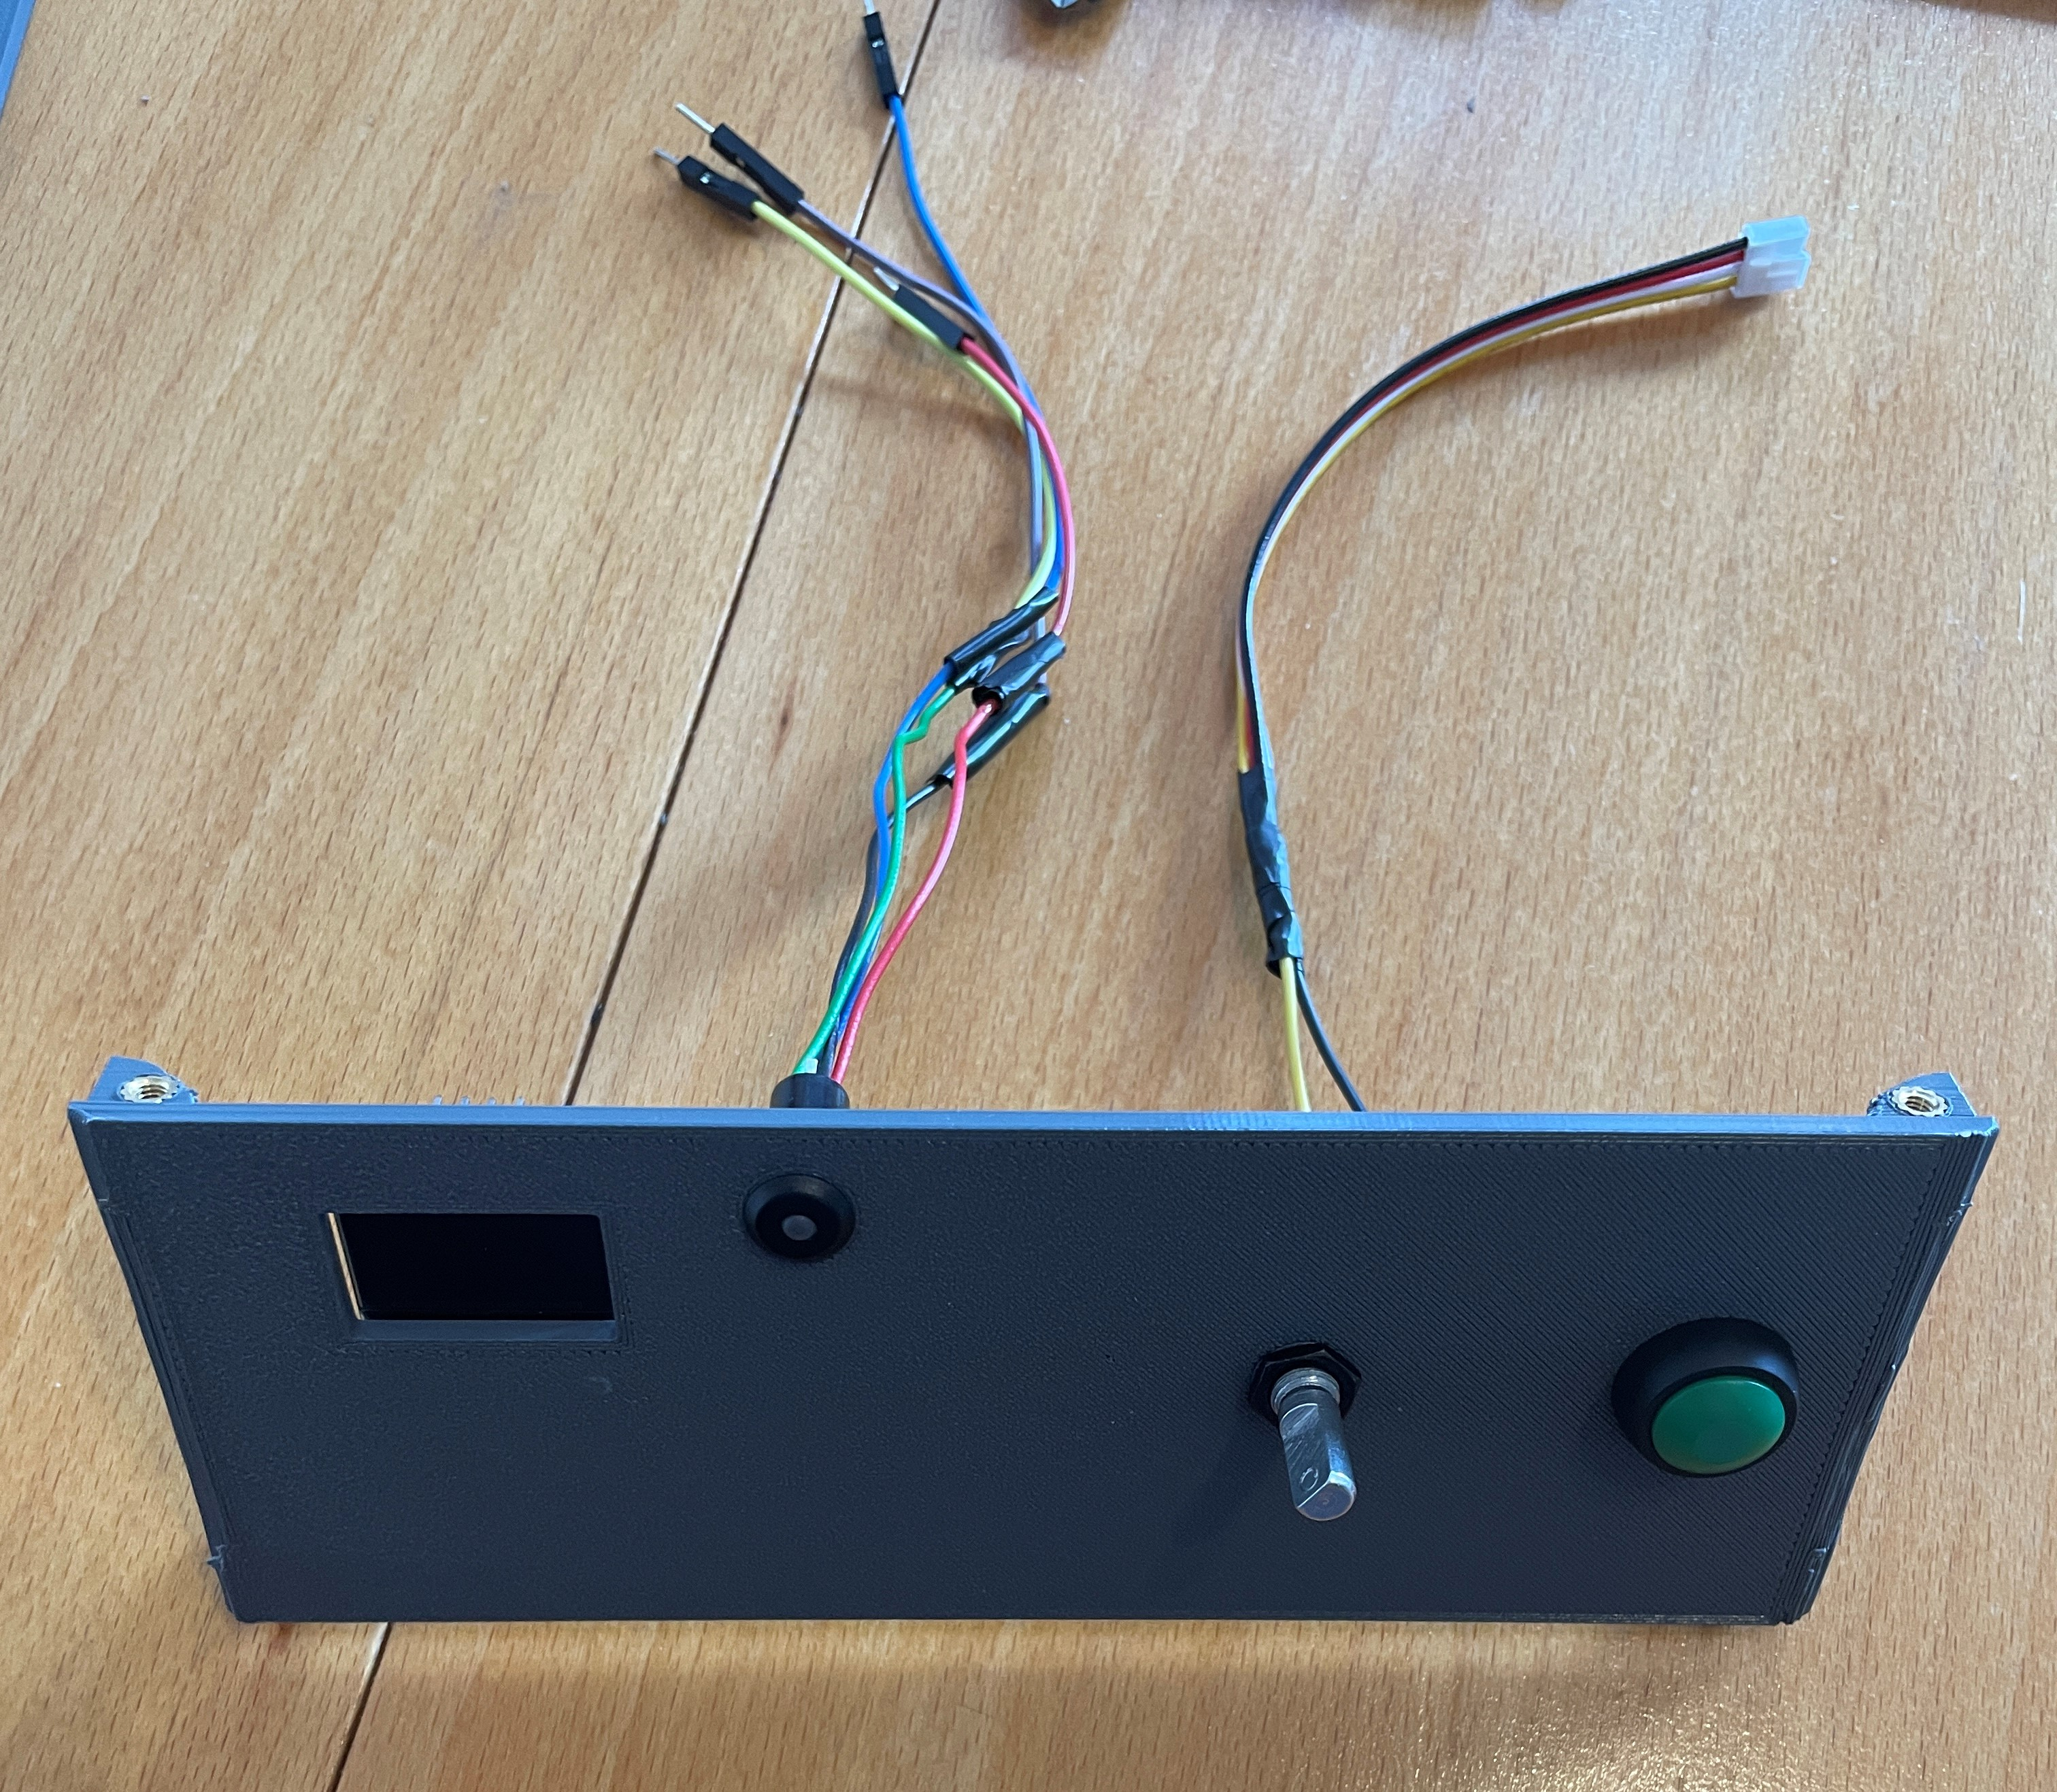
\includegraphics[width=\textwidth]{Images/3Schr.jpg}
		\caption{Dritter Schritt: Zusammenbau der Vorderplatte} \label{3.S}
	\end{center}
\end{figure}


\section{Vierter Schritt: Zusammenbau der Hinterplatte}
Montieren Sie die folgenden Bauteile und elektrischen Komponenten wie in Abbildung \ref{4.S} gezeigt. 

\begin{enumerate}
	\item Montieren Sie den Kaltgeräteanschluss an der Hinterplatte. Ein Klickgeräusch bestätigt den korrekten Sitz.
\end{enumerate}

\begin{figure}[H]
	\begin{center}
		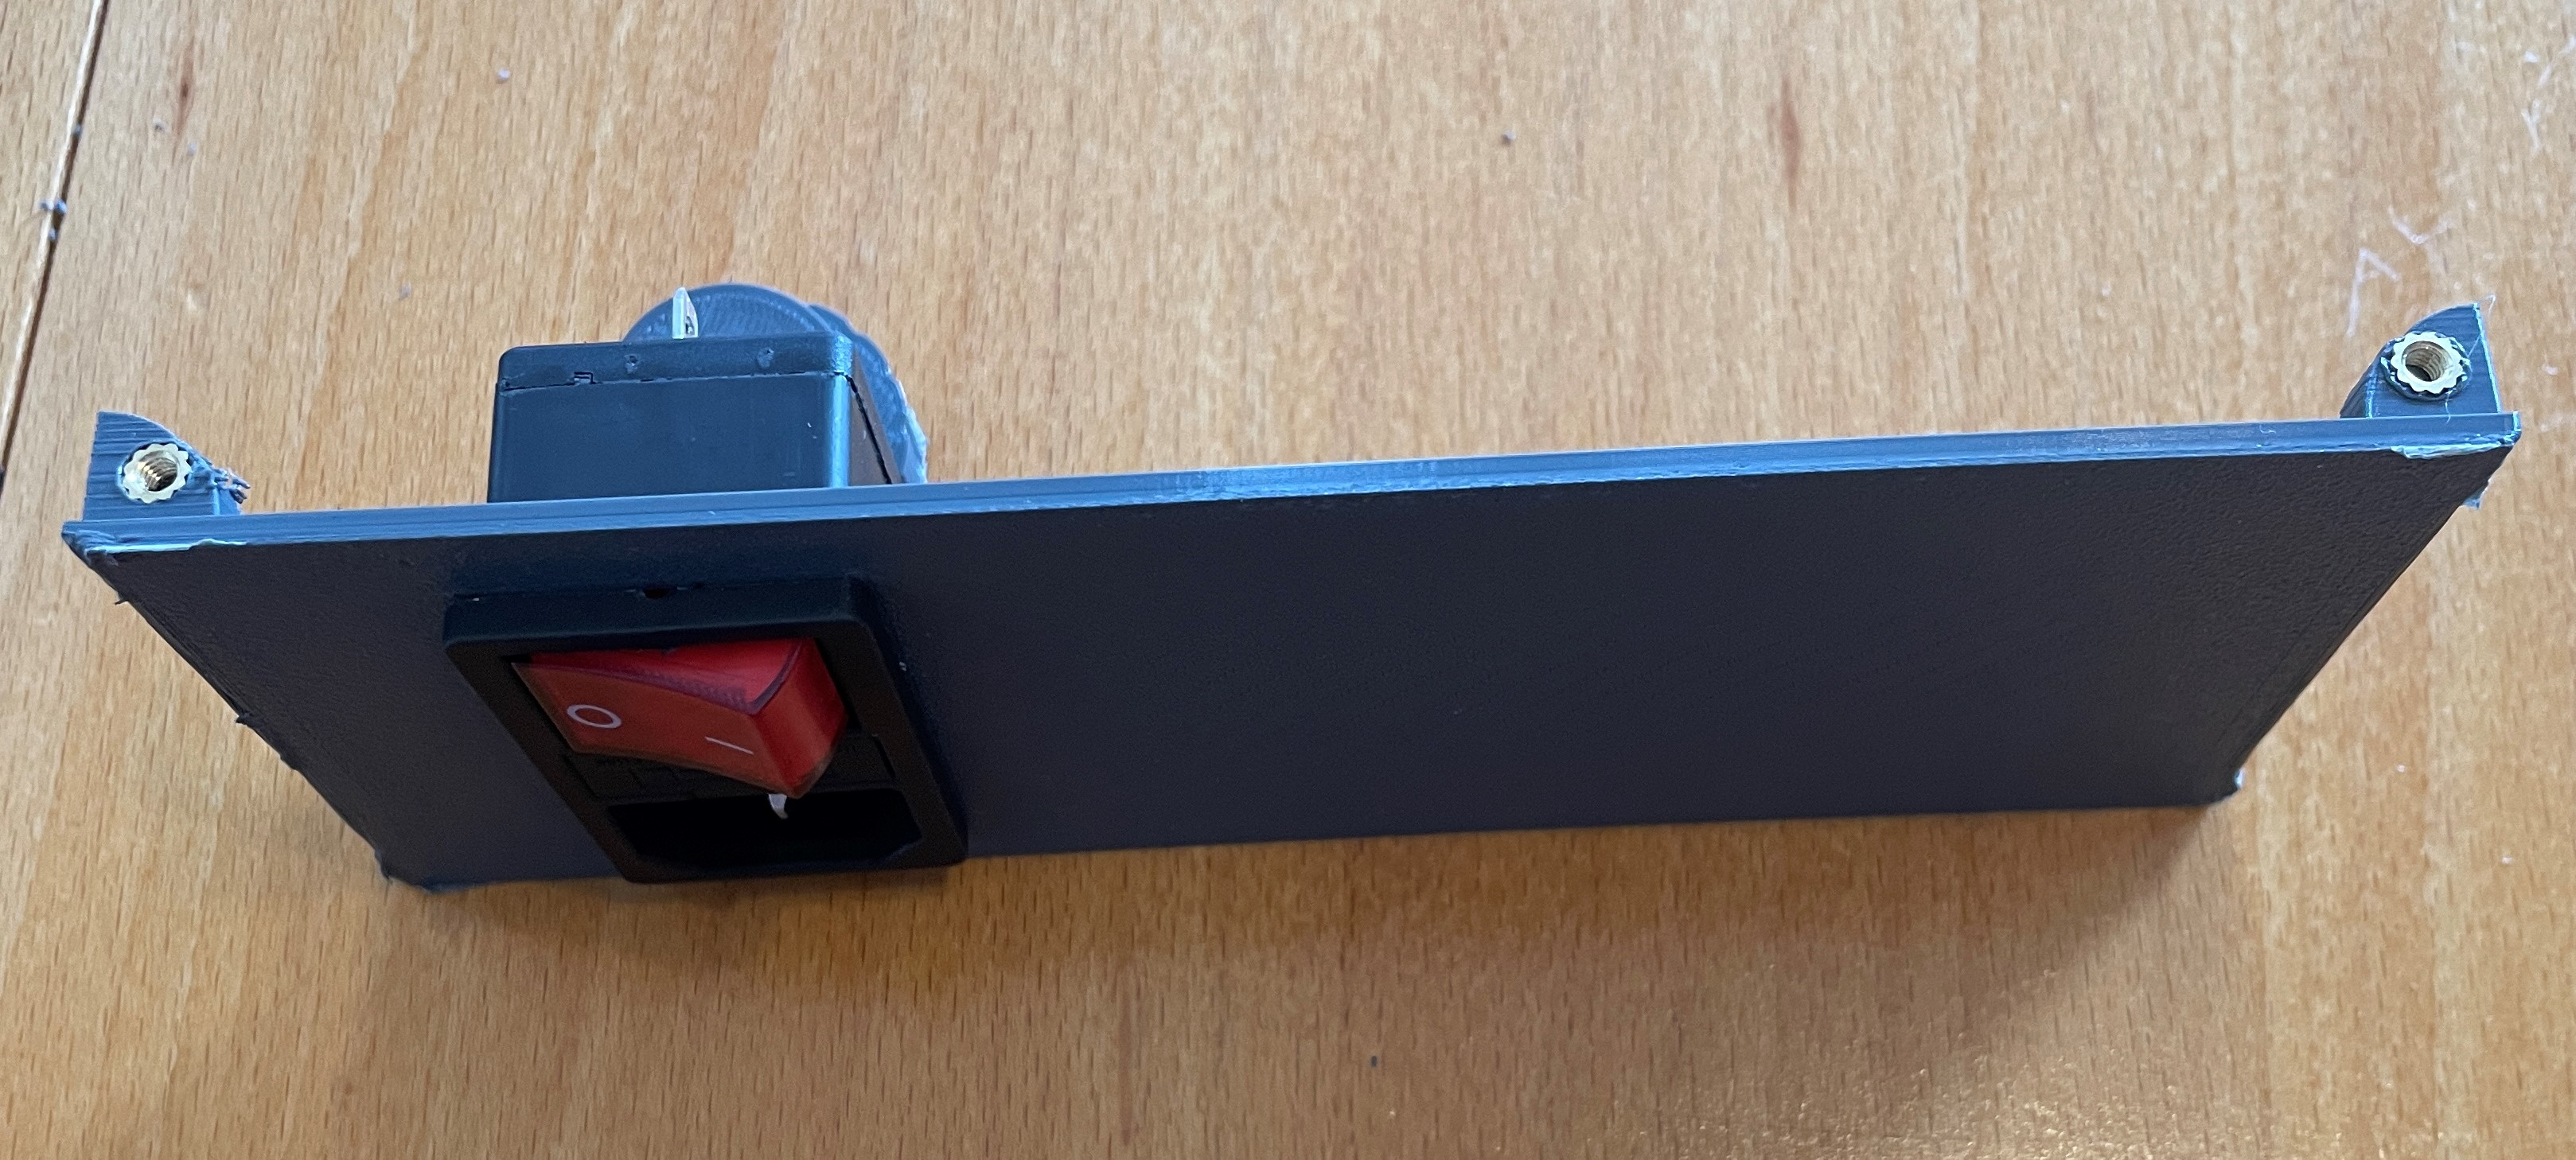
\includegraphics[width=\textwidth]{Images/4Schr.jpg}
		\caption{Vierter Schritt: Zusammenbau der Hinterplatte} \label{4.S}
	\end{center}
\end{figure}


\section{Fünfter Schritt: Teilzusammenbau des Gehäuses}
Montieren Sie die folgenden Bauteile und elektrischen Komponenten wie in Abbildung \ref{5.S} gezeigt. 

\begin{enumerate}
	\item Verschrauben Sie die Vorderplatte und die Hinterplatte mit der Bodenplatte. Verwenden Sie dafür 4 $\times$ $ M3 \times 10 \ mm $ Schrauben.
	\item Befestigen Sie die rechte Seitenplatte mit der Vorder- und Hinterplatte. Verwenden Sie dafür 2 $\times$ $ M3 \times 10 \ mm $ Schrauben.
\end{enumerate}

\begin{figure}[H]
	\begin{center}
		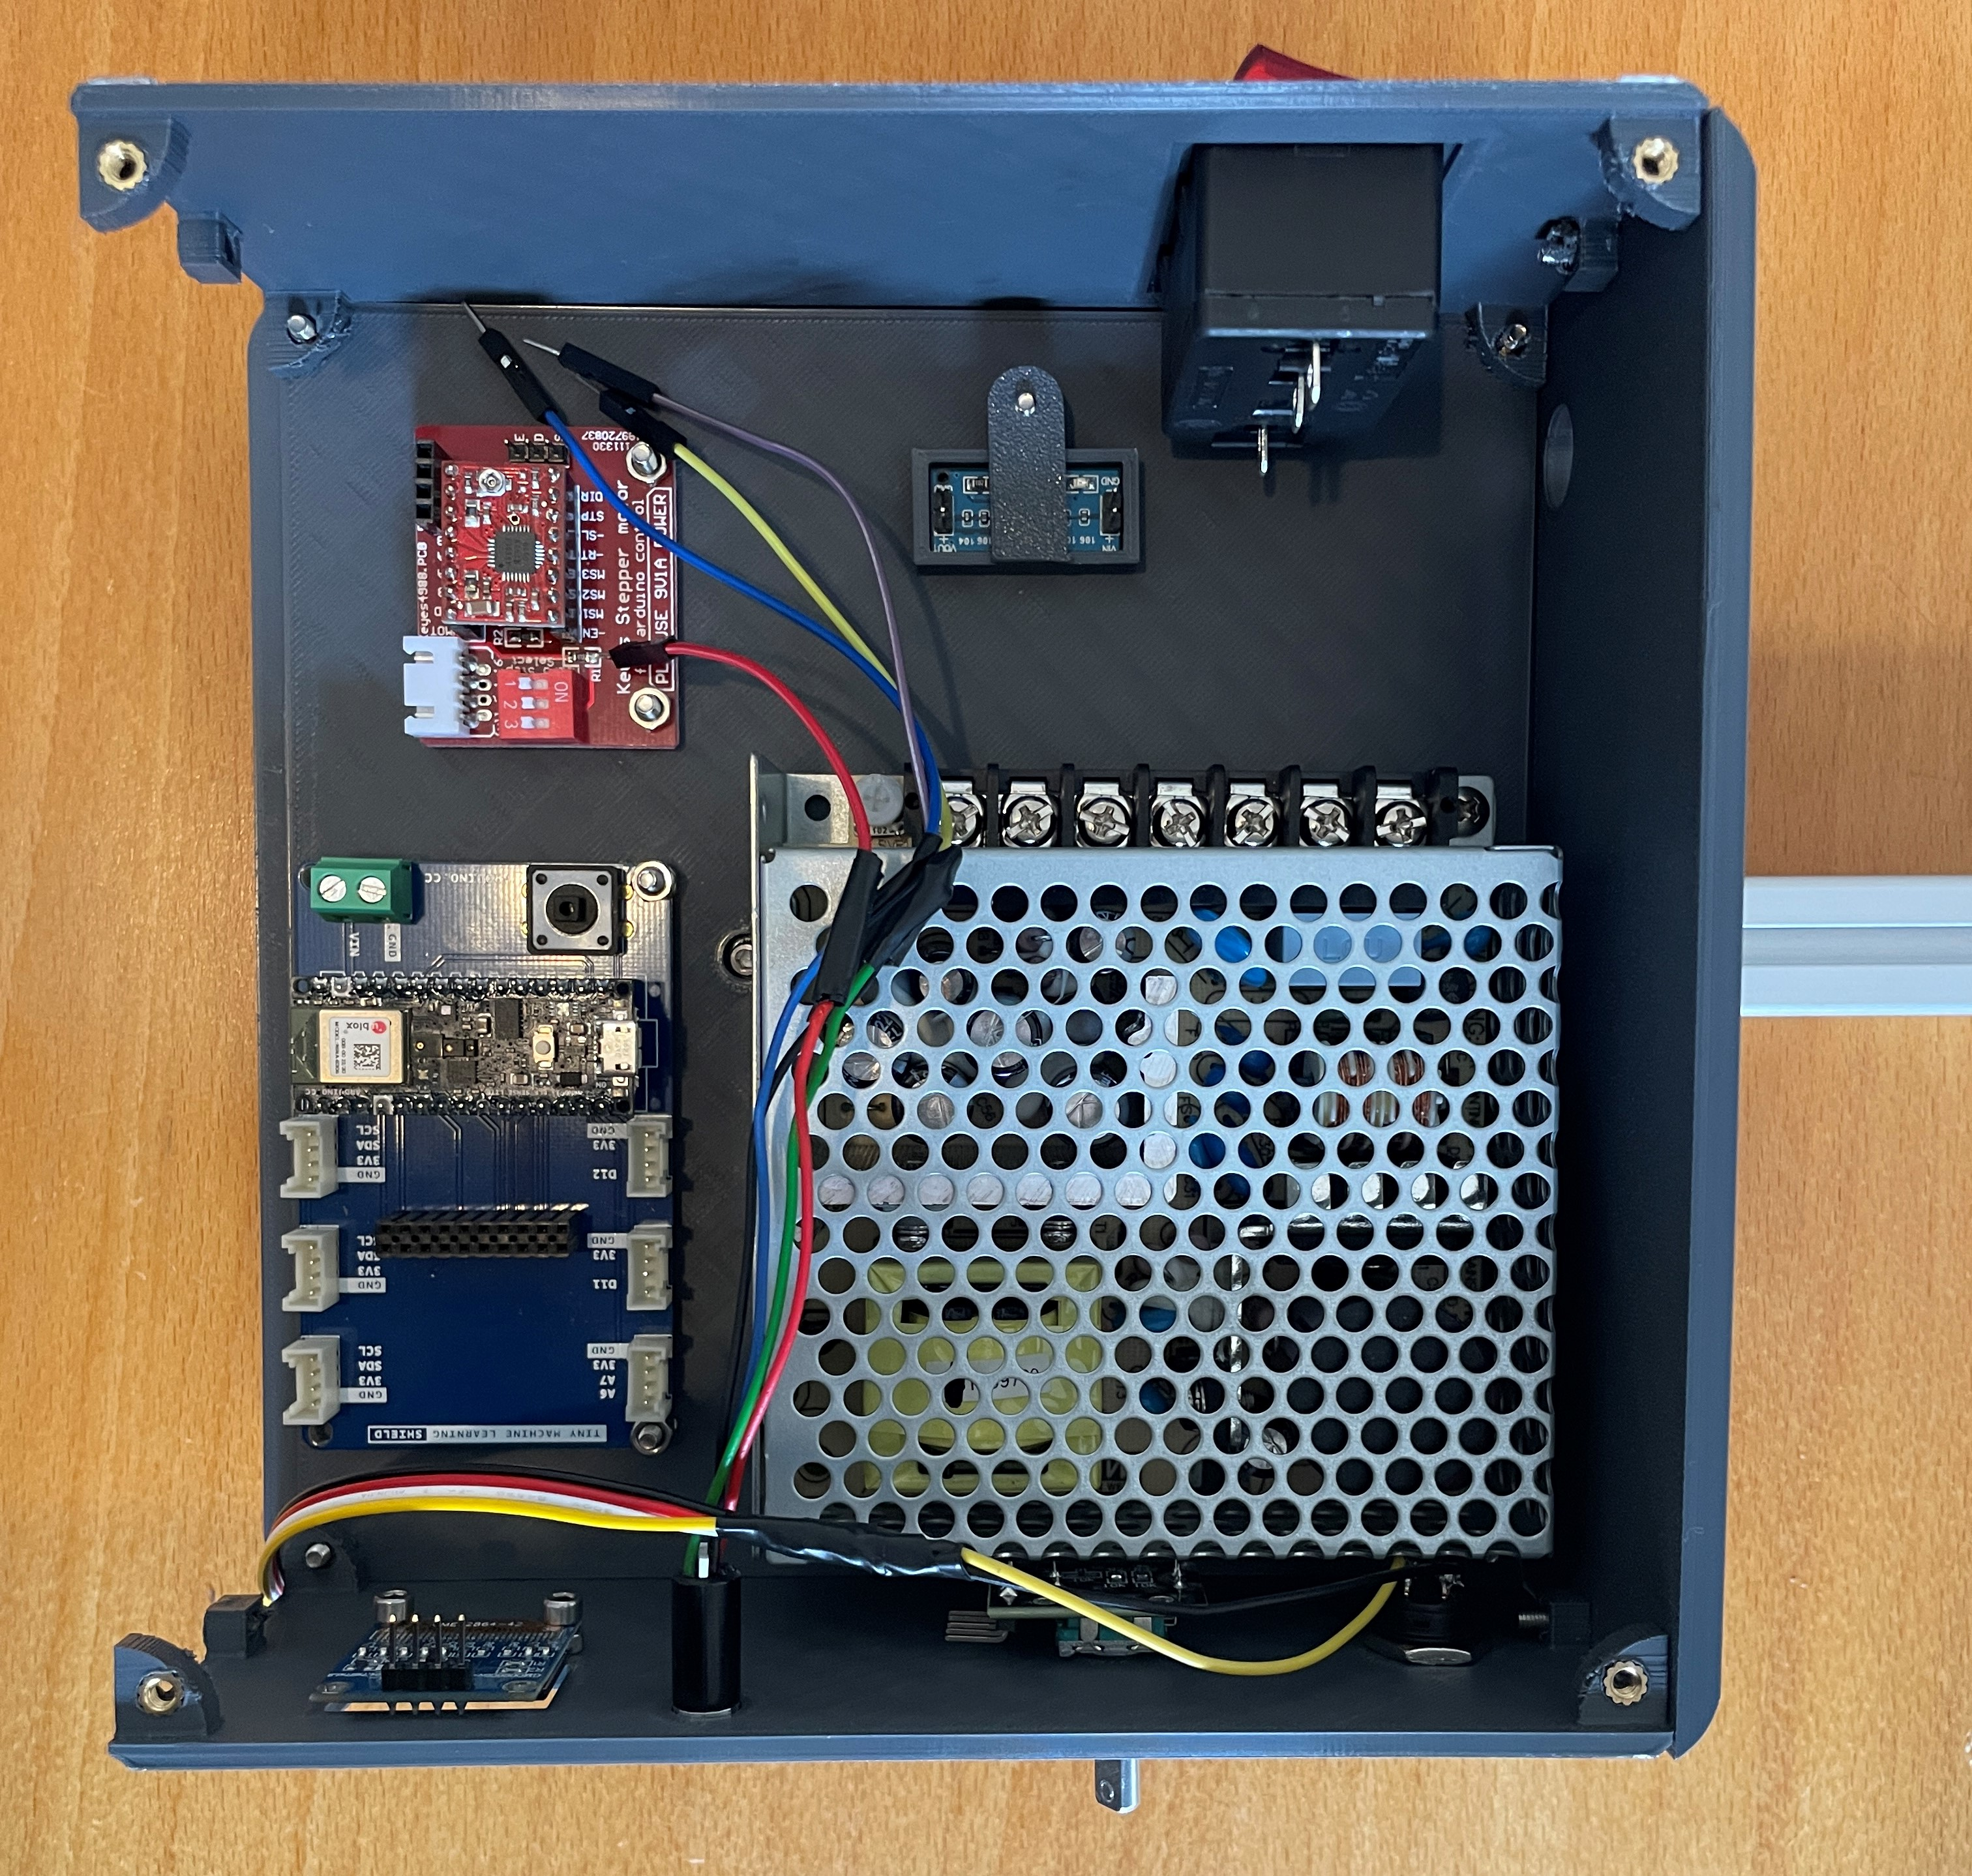
\includegraphics[width=\textwidth]{Images/5Schr.jpg}
		\caption{Fünfter Schritt: Teilzusammenbau des Gehäuses} \label{5.S}
	\end{center}
\end{figure}


\section{Sechster Schritt: Anschließen der elektrischen Leitungen}

\begin{enumerate}
	\item Verbinden Sie die Leitungen gemäß dem Schaltplan (siehe Abbildung \ref{Splan}). Dieser Schritt sollte von einer Elektrofachkraft durchgeführt oder überprüft werden.
	\item Führen Sie die Leitungen für den Motor und den Micro-Schalter durch die Öffnung in der rechten Seitenplatte.
\end{enumerate}

\begin{figure}[H]
	\begin{center}
		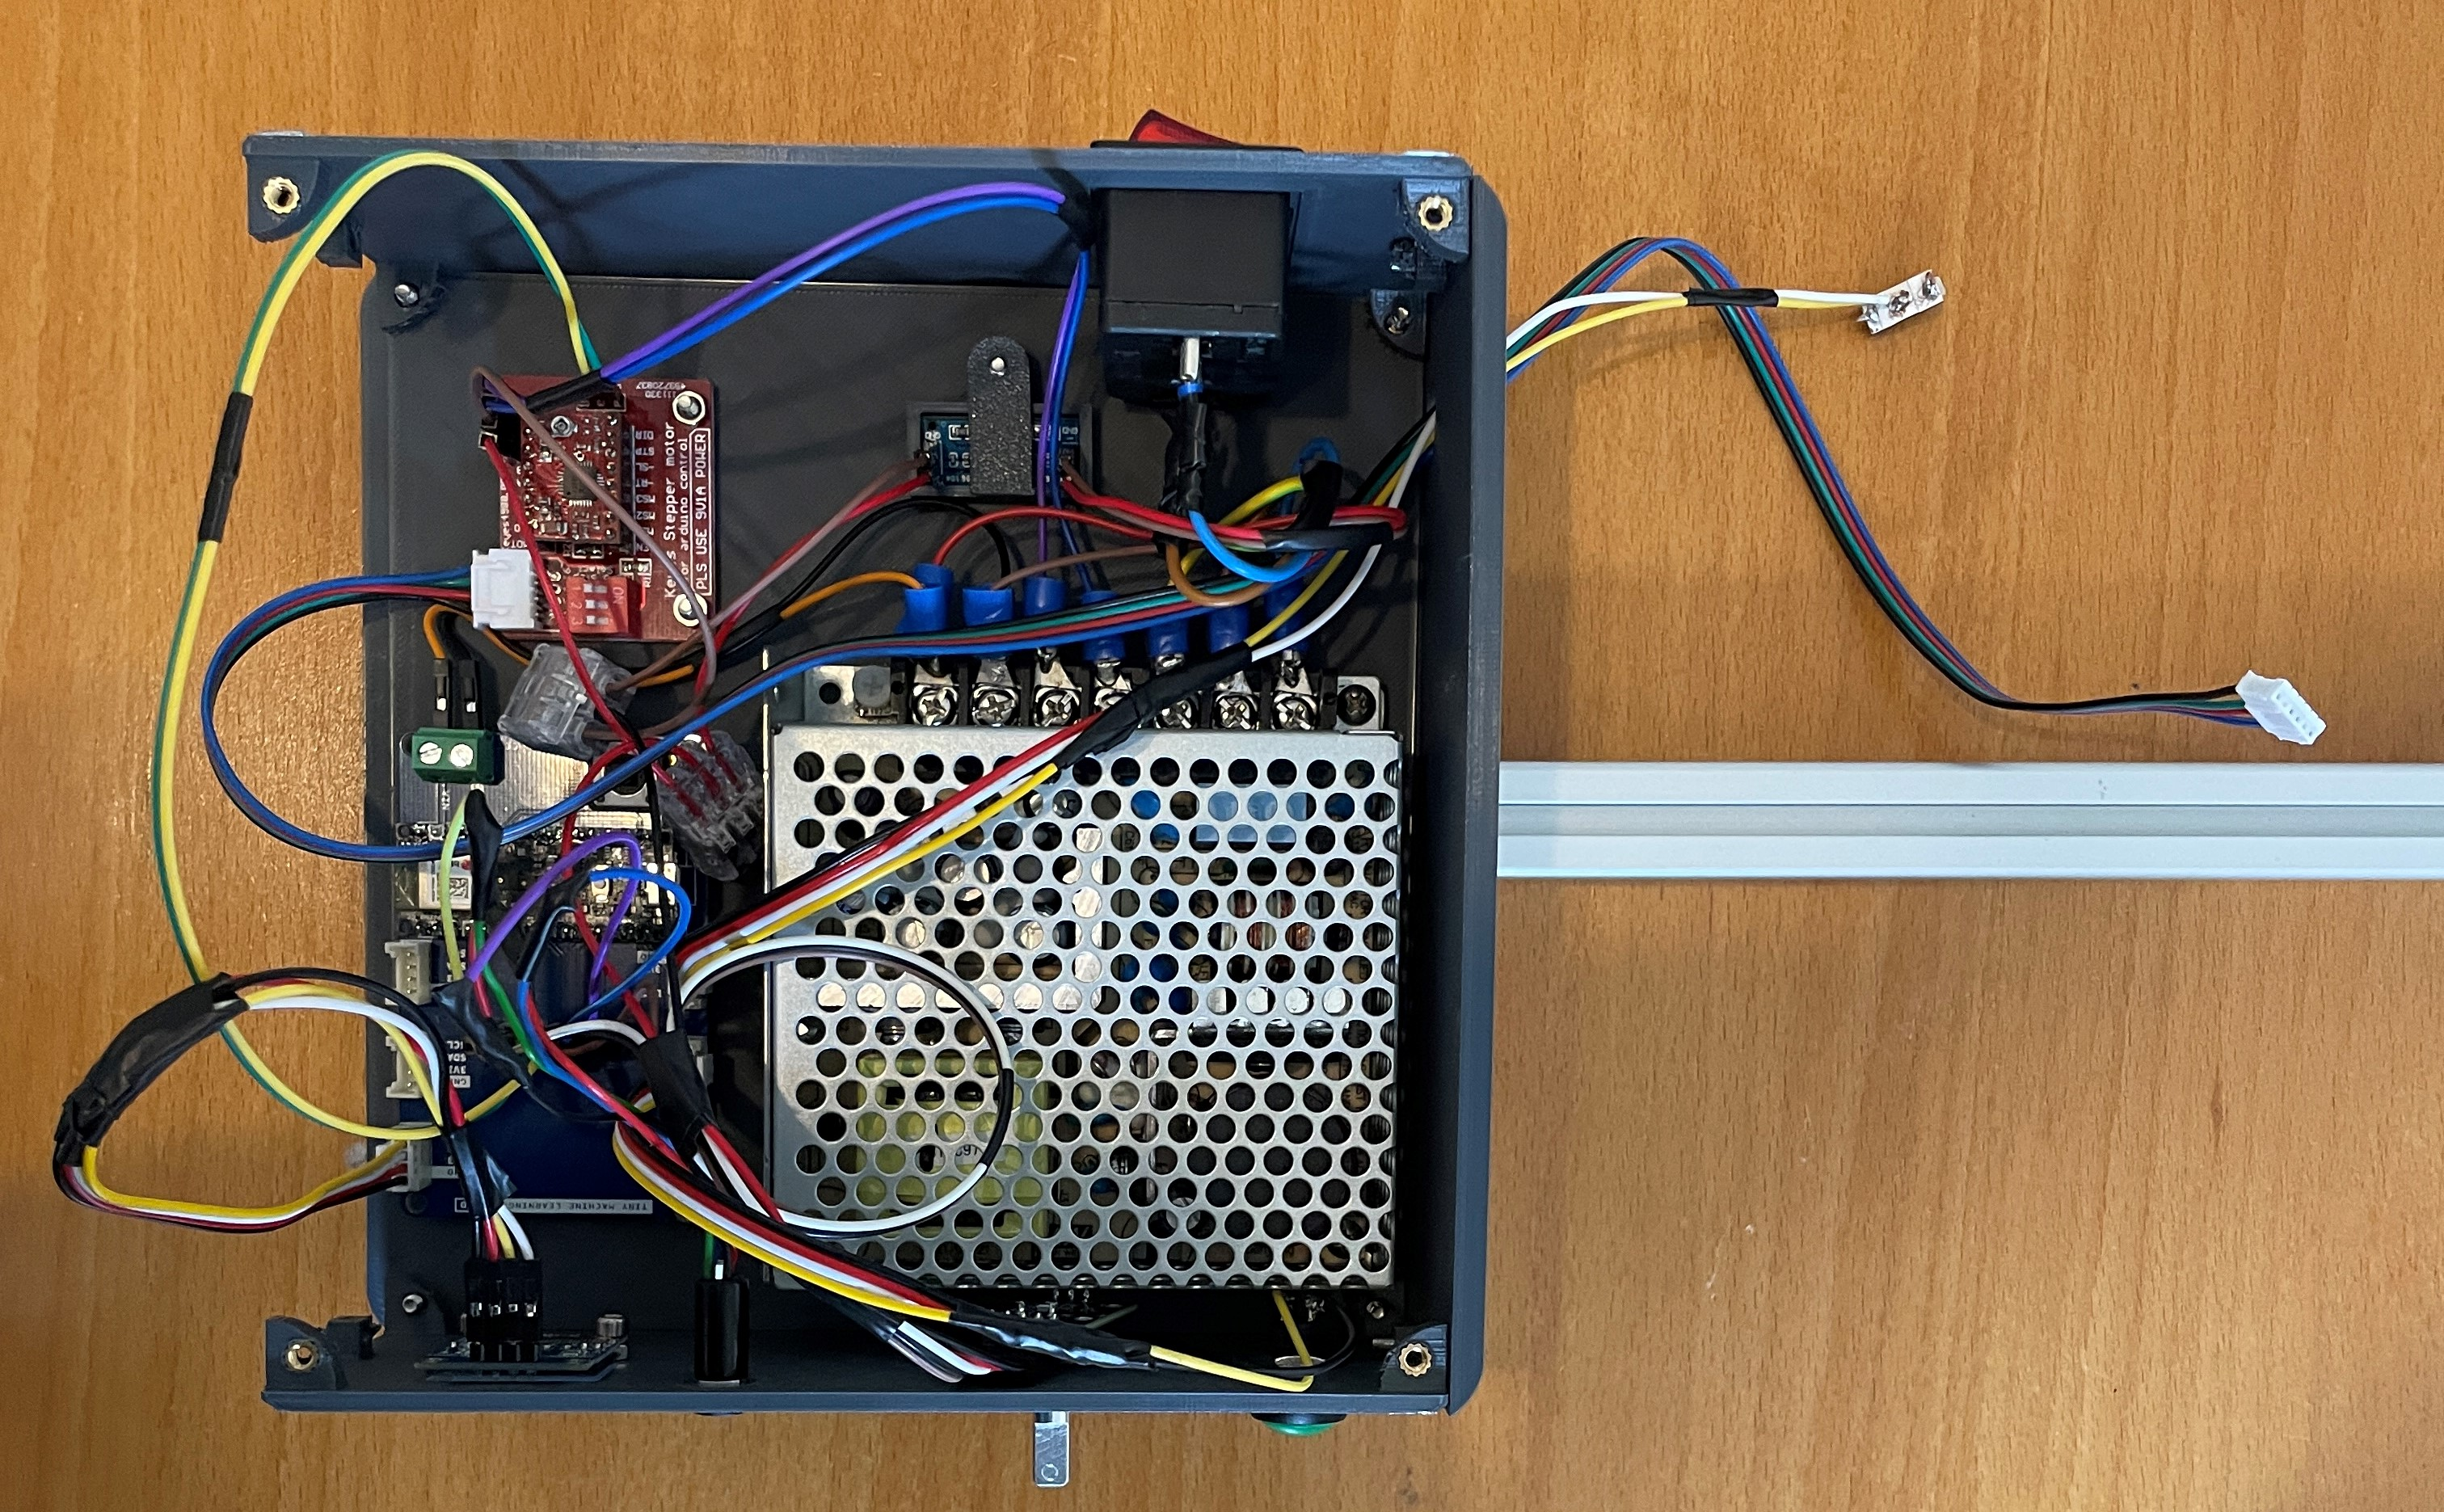
\includegraphics[width=\textwidth]{Images/6Schr.jpg}
		\caption{Schaltplan} \label{6.S}
	\end{center}
\end{figure}


\section{Siebter Schritt: Montieren des Micro-Schalters und Motors}
Montieren Sie die folgenden Bauteile und elektrischen Komponenten wie in Abbildung \ref{7.S} gezeigt.

\begin{enumerate}
	\item Befestigen Sie den Micro-Schalter mit 2 $\times$ $ M2.5 \times 6 \ mm $ Schrauben an der Halterung für den Motor.
	\item Montieren Sie den Nema 17 Motor an der Halterung für die Welle mit 4 $\times$ $ M3 \times 6 \ mm  $ Schrauben.
	\item Führen Sie 2 $\times$ $ M3 $ Hammermutter in das Aluprofil ein.
	\item Befestigen Sie die Halterung am Aluprofil mit 2 $\times$ $ M3 \times 8 \ mm $ und 2 $\times$ $ M3 $ Hammermuttern. Halten Sie einen Abstand vom Gehäuse von ca. 15 bis 20 \ mm. 
	\item Verbinden Sie die Leitung für den Motor an dem Motor. 
\end{enumerate}

\begin{figure}[H]
	\begin{center}
		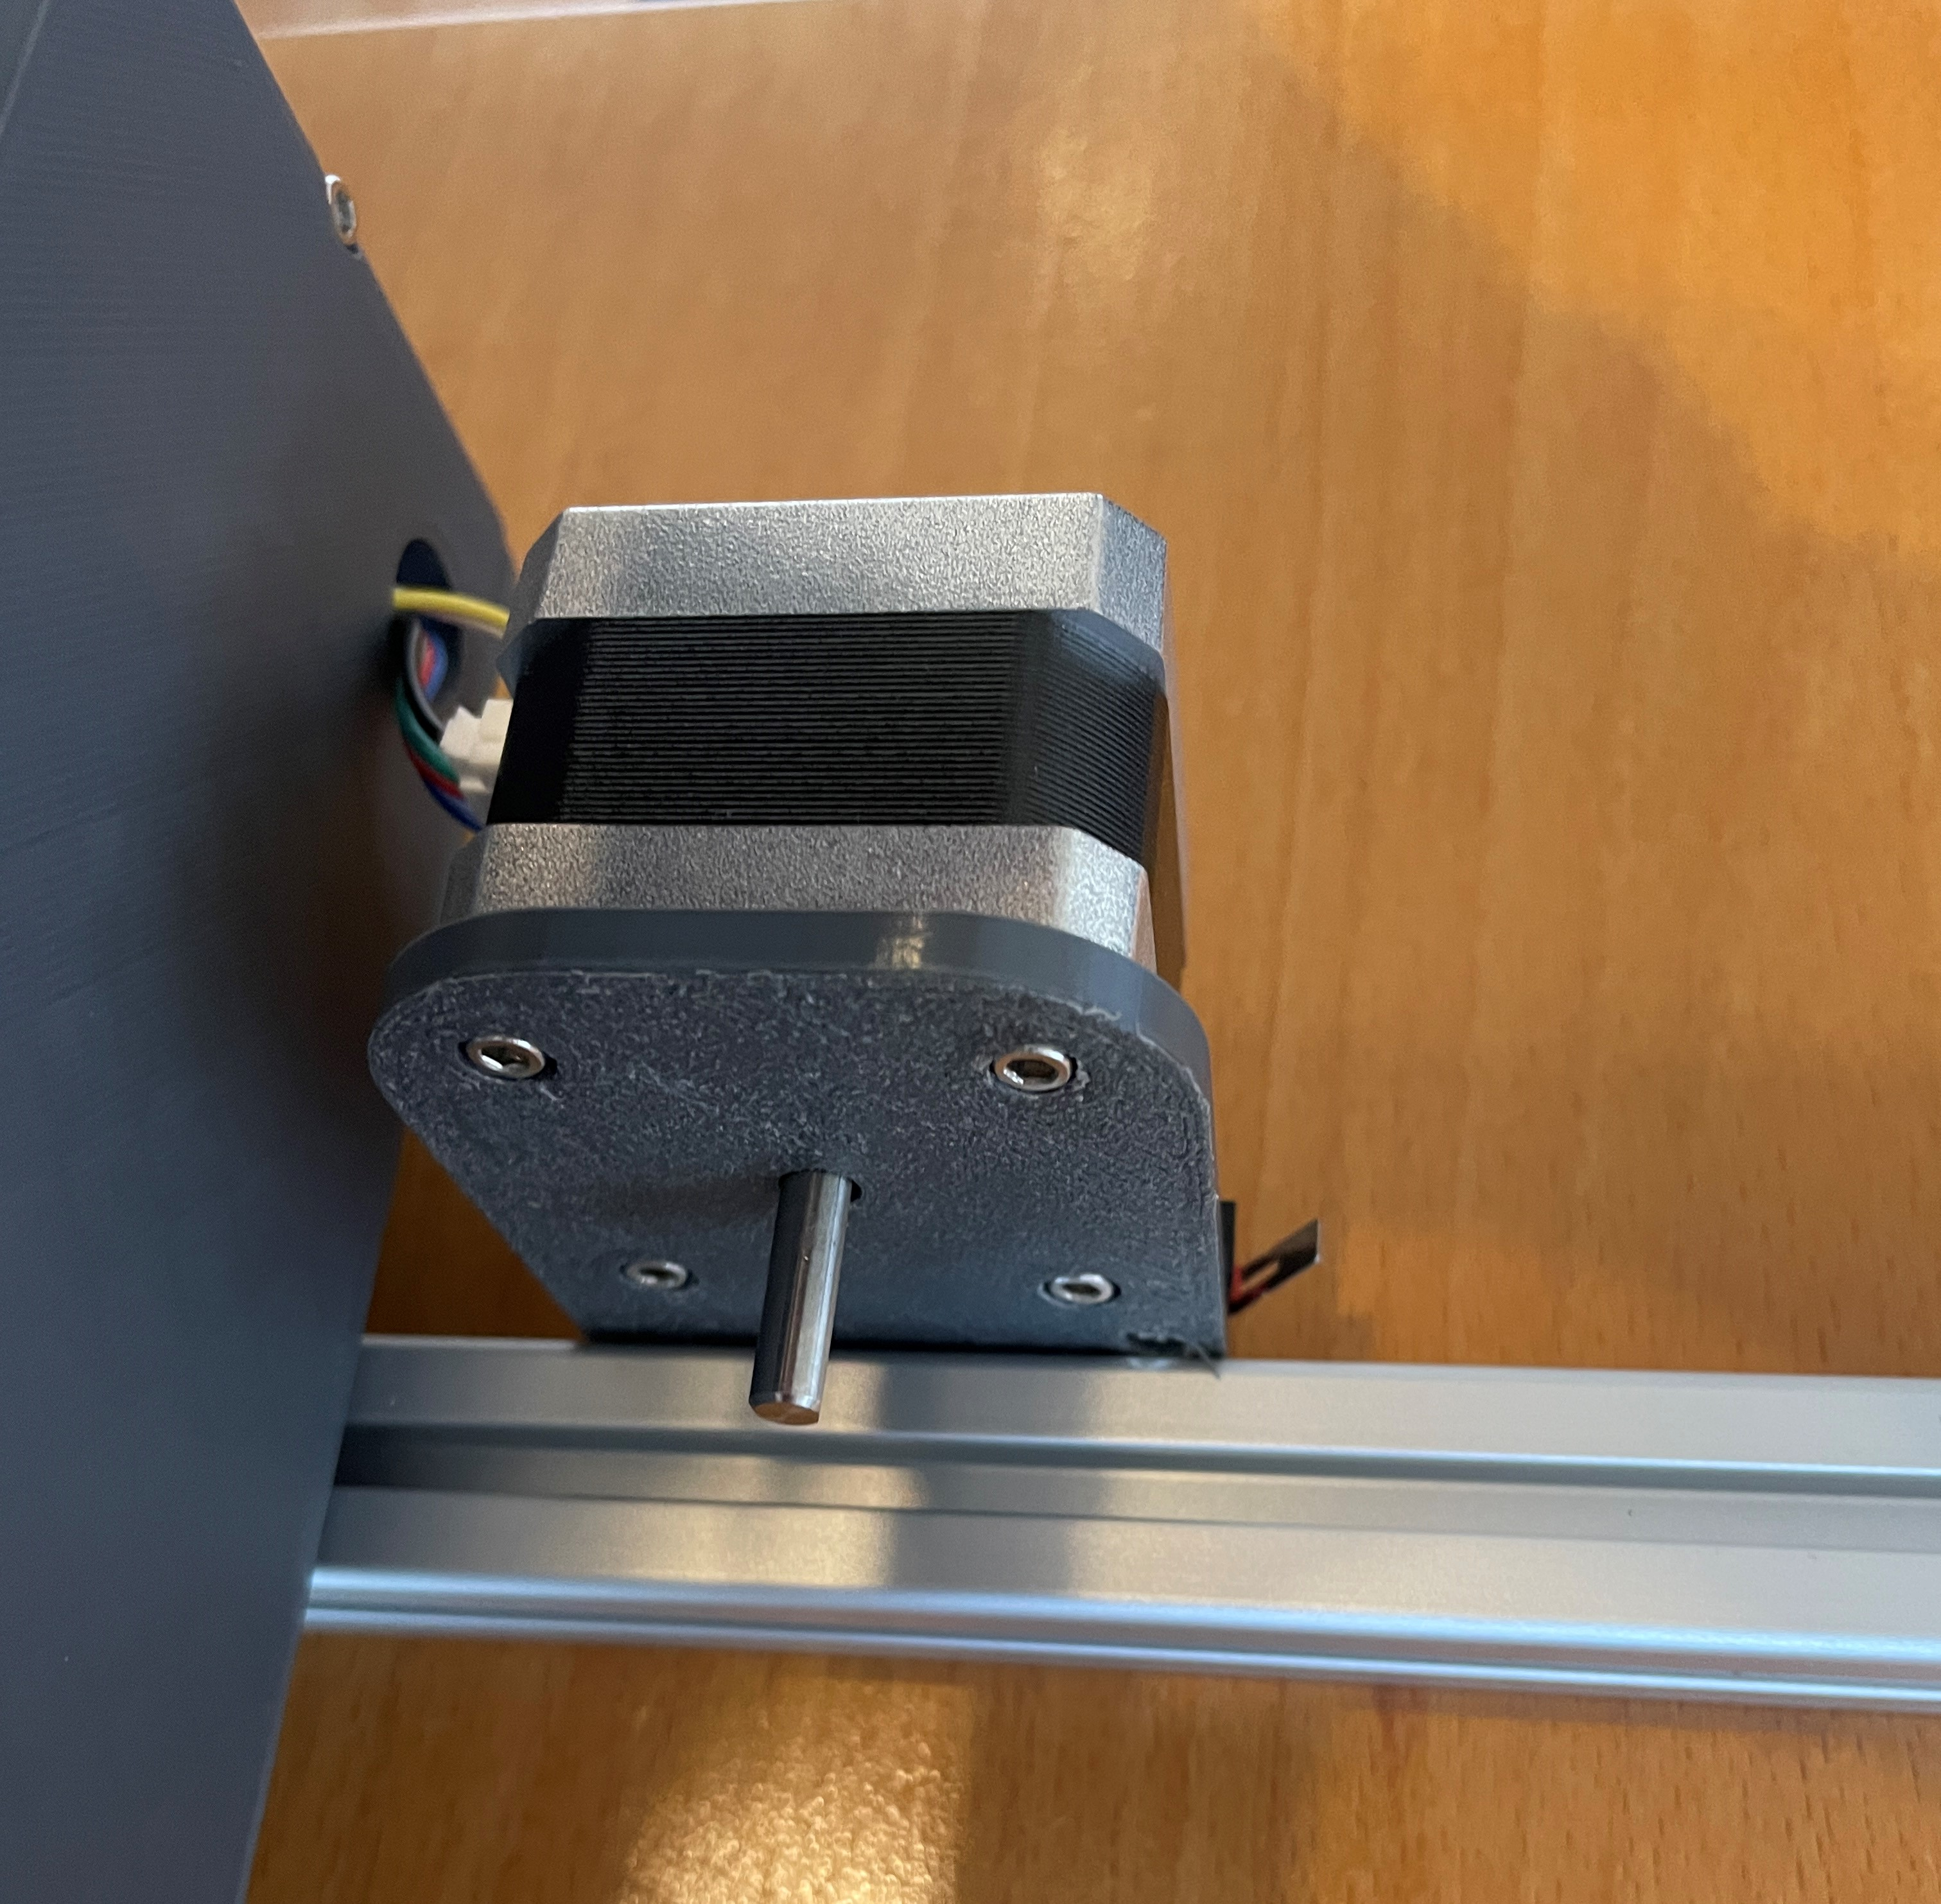
\includegraphics[width=\textwidth]{Images/7Schr.jpg}
		\caption{Siebter Schritt: Montieren des Micro-Schalters und Motors} \label{7.S}
	\end{center}
\end{figure}


\section{Achter Schritt: Zusammenbau des Gehäuses}
Montieren Sie die folgenden Bauteile und elektrischen Komponenten wie in Abbildung \ref{8.S} gezeigt.

\begin{enumerate}
	\item Verschrauben Sie die Seitenplatte Links und die Hinterplatte mit der Vorderplatte und Hinterplatte. Verwenden Sie dafür 2 $\times$ $ M3 \times 10 \ mm $ Schrauben.
	\item Verschrauben Sie die Deckelplatte mit der Vorderplatte und Hinterplatte. Verwenden Sie dafür 4 $\times$ $ M3 \times 10 \ mm $ Schrauben.
\end{enumerate}

\begin{figure}[H]
	\begin{center}
		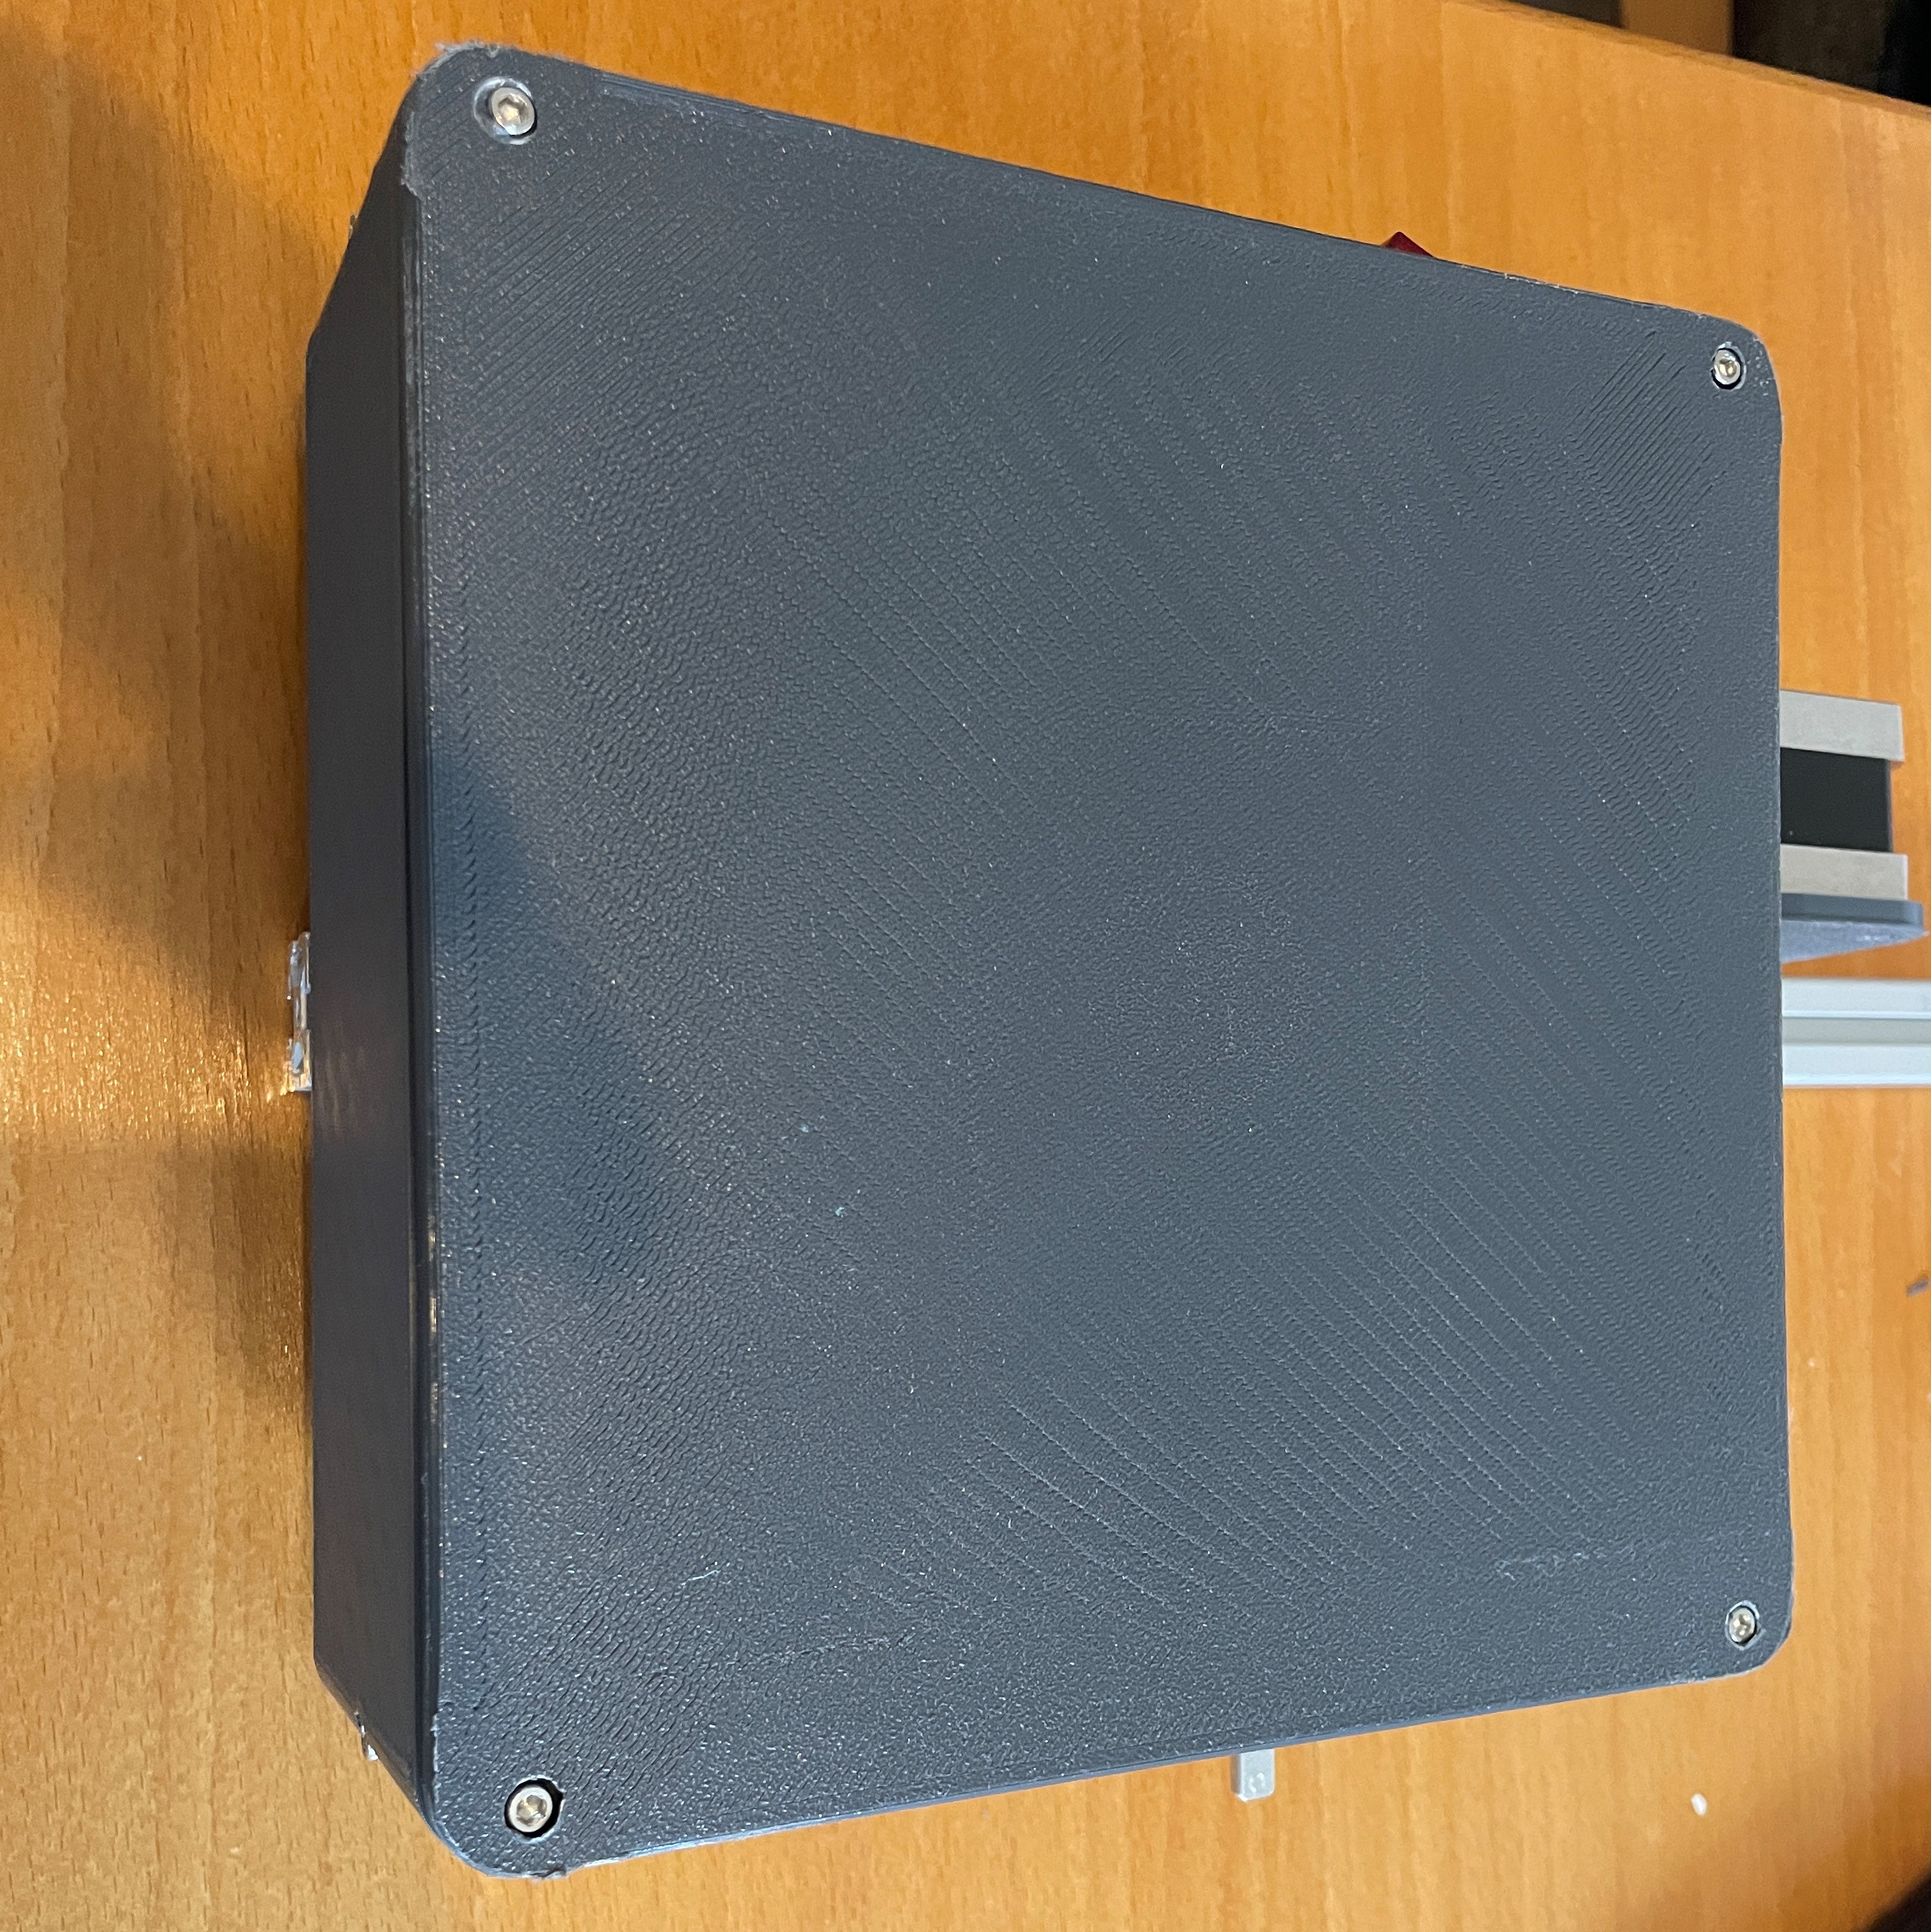
\includegraphics[width=\textwidth]{Images/8Schr.jpg}
		\caption{Achter Schritt: Zusammenbau des Gehäuses} \label{8.S}
	\end{center}
\end{figure}

\section{Neunter Schritt: Montieren der Linearführung}
Montieren Sie die folgenden Bauteile wie in Abbildung \ref{9.S} gezeigt.

\begin{enumerate}
	\item Führen Sie 5 $\times$ $ M3 $ Hammermutter in das Aluprofil ein.
	\item Befestigen Sie die Liniearführung am Aluprofil mit 5 $\times$ $ M3 \times 10 \ mm $ und 5 $\times$ $ M3 $ Hammermuttern. Lassen Sie an jeder Seite eine Bohrung frei und nutzen Sie dann jede fünfte Bohrung. 
\end{enumerate}

\begin{figure}[H]
	\begin{center}
		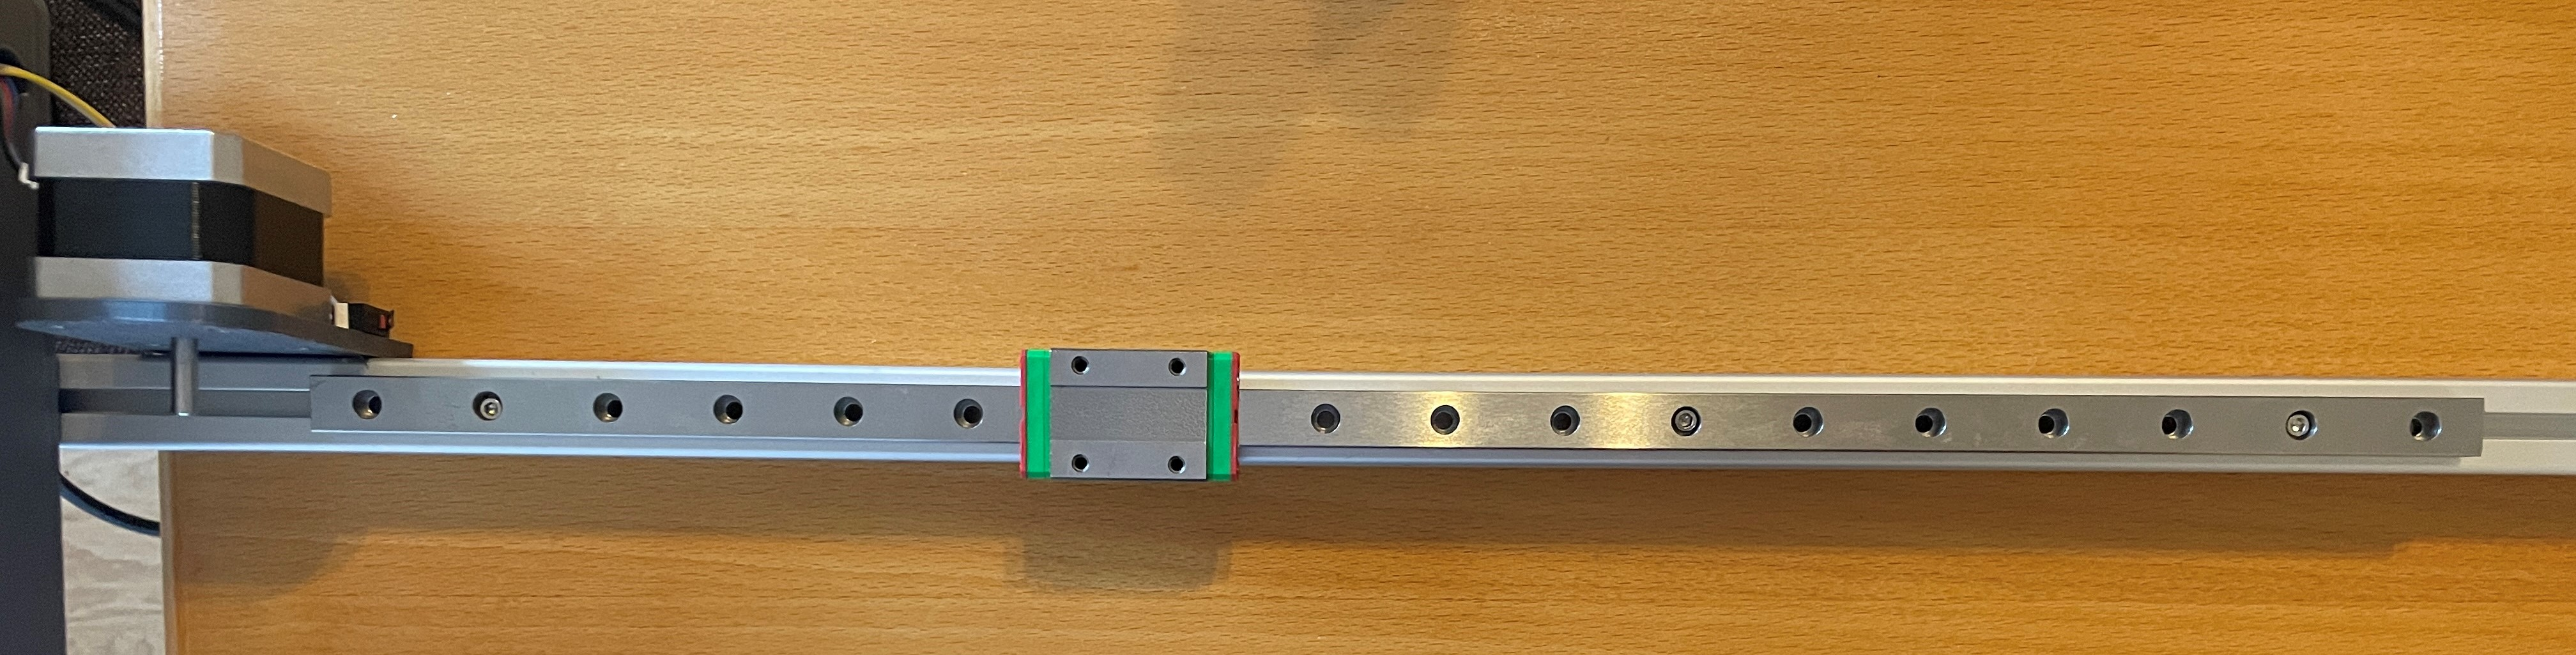
\includegraphics[width=\textwidth]{Images/9Schr.jpg}
		\caption{Neunter Schritt: Montage der Liniearführung} \label{9.S}
	\end{center}
\end{figure}

\section{Zehnter Schritt: Montieren des Griffs}
Montieren Sie die folgenden Bauteile wie in Abbildung \ref{10.S} gezeigt.

\begin{enumerate}
	\item Führen Sie 2 $\times$ $ M3 $ Hammermutter in das Aluprofil ein.
	\item Montieren Sie den Anzeiger auf den Schlitten der Liniearführung mit 4 $\times$ $ M3 \times 6 \ mm $ Schrauben.
	\item Montieren Sie den Riemen Auf den Anzeiger mit 4 $\times$ $ M3 \times 6 \ mm $ Schrauben.
\end{enumerate}

\begin{figure}[H]
	\begin{center}
		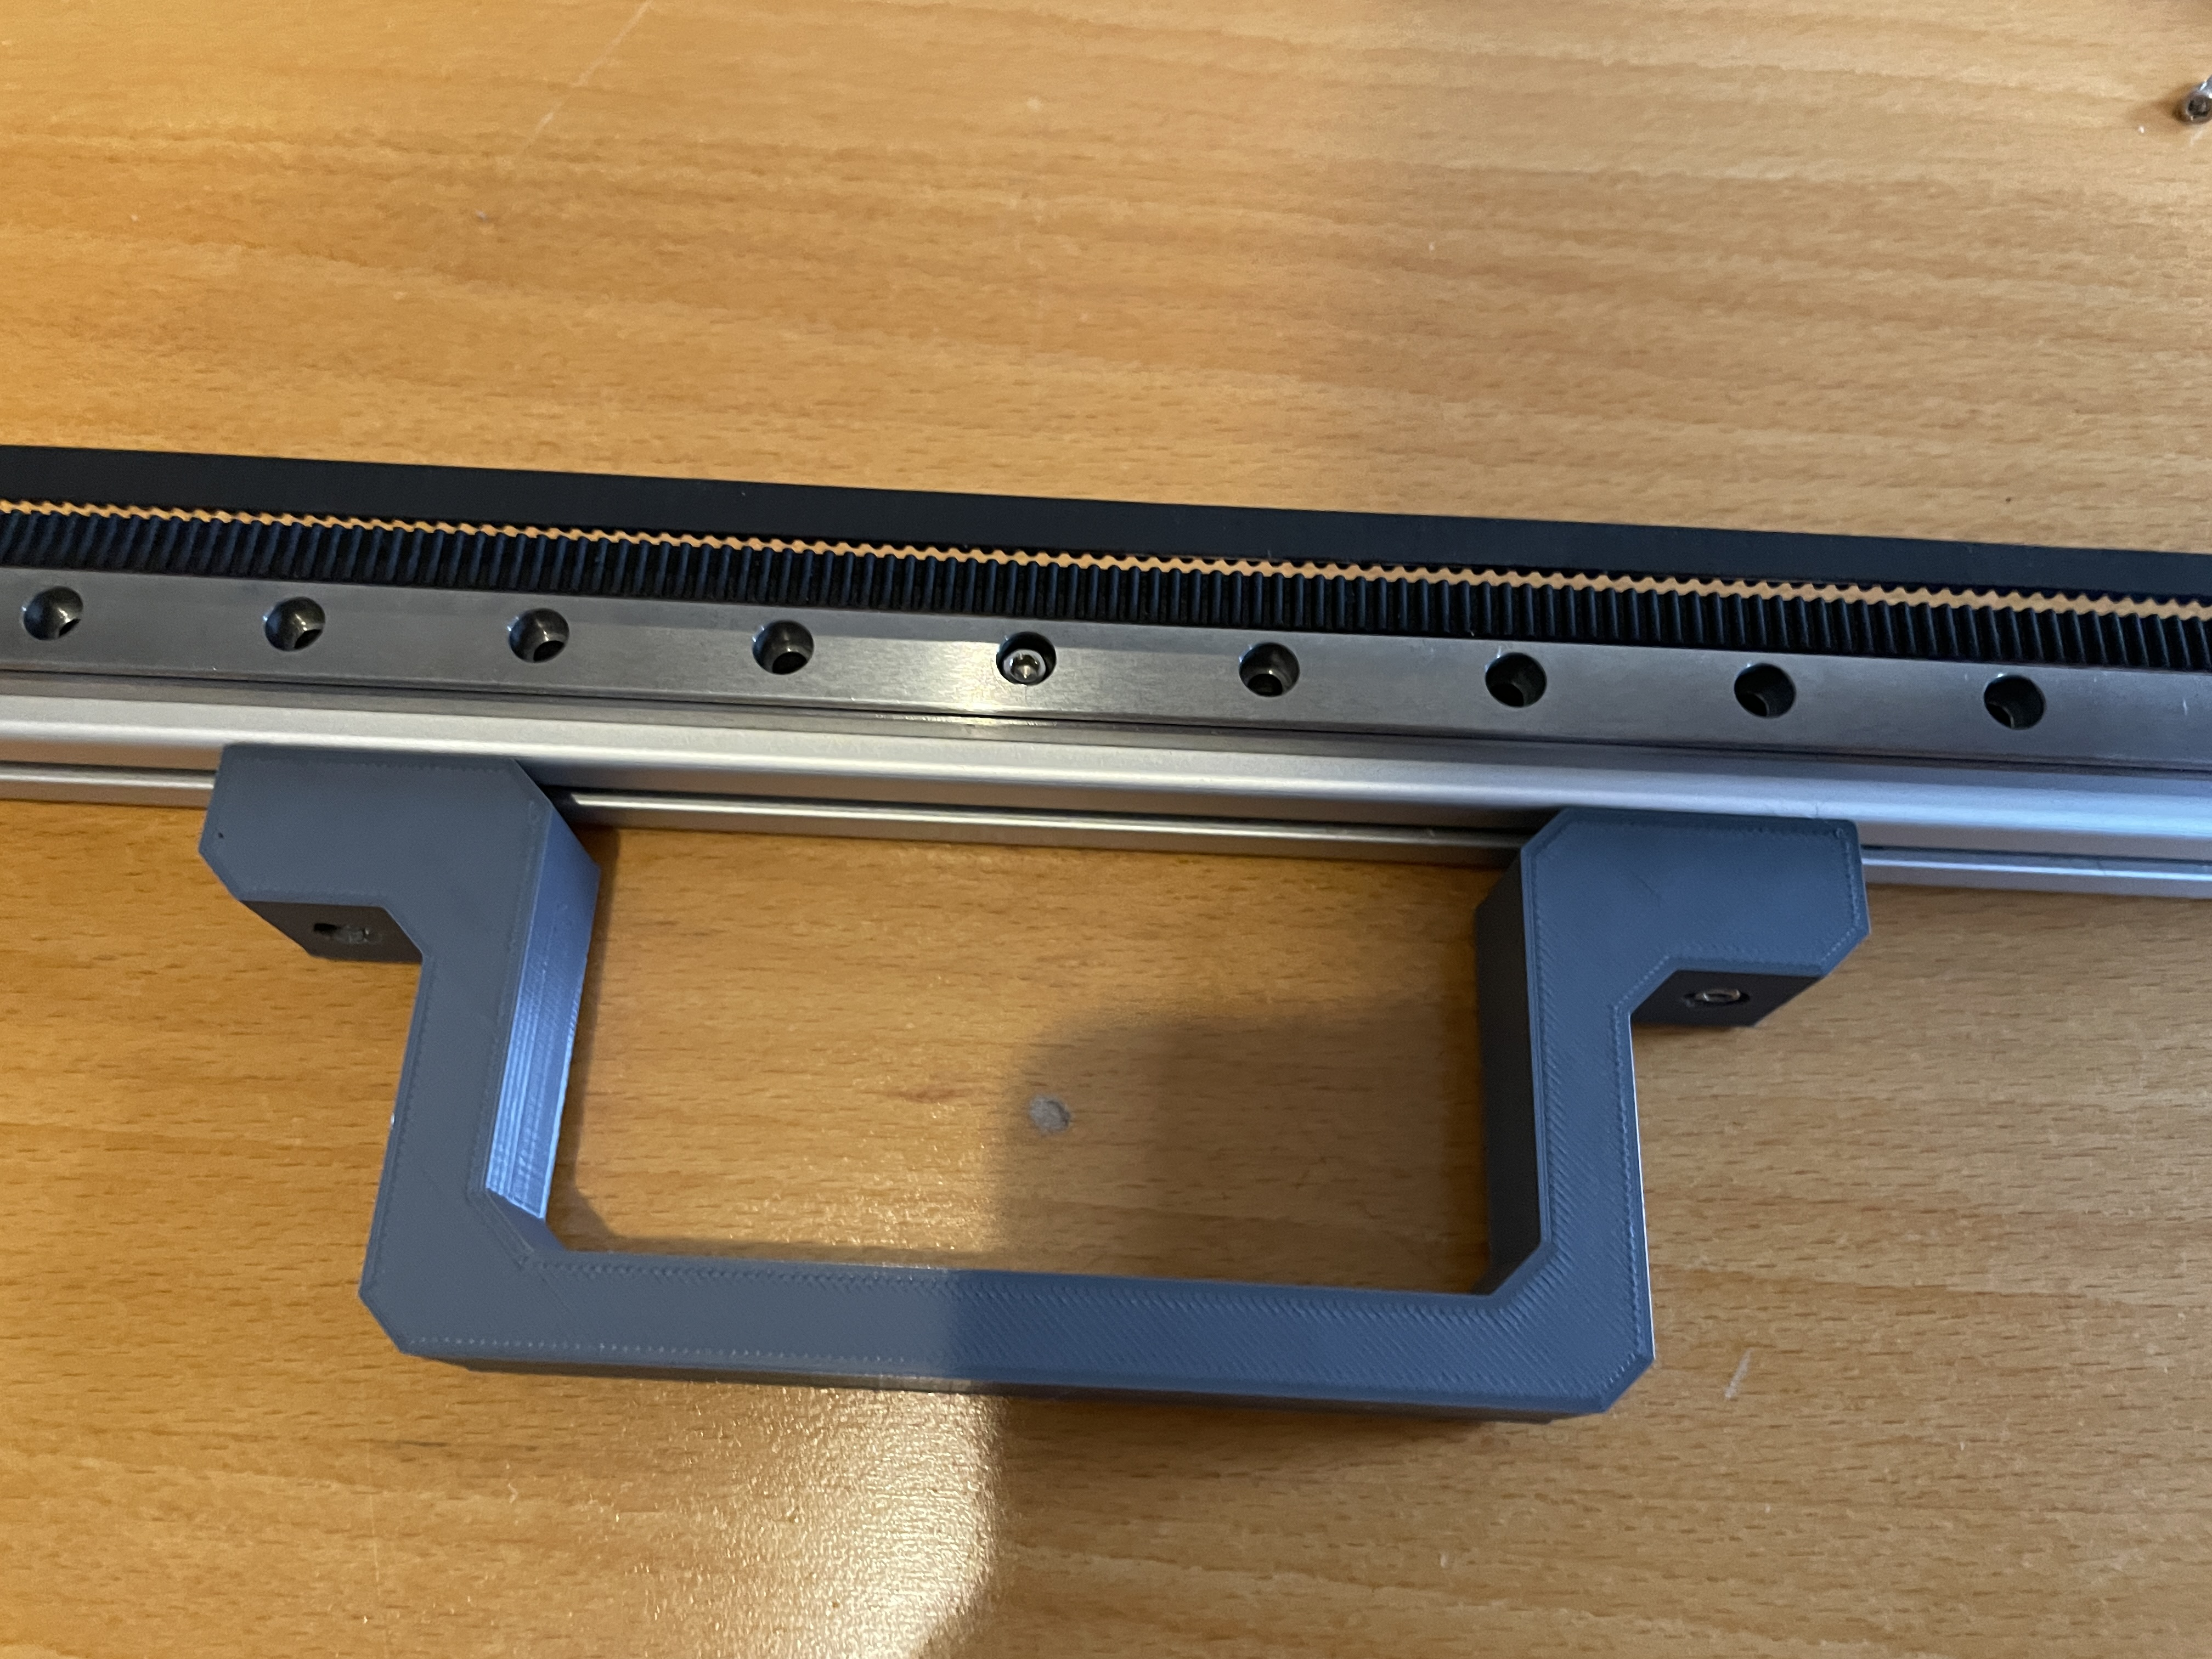
\includegraphics[width=\textwidth]{Images/10Schr.jpg}
		\caption{Dreizehnter Schritt:Montieren des Griffs} \label{10.S}
	\end{center}
\end{figure}


\section{Elfter Schritt: Montieren der Halter für die Welle}
Montieren Sie die folgenden Bauteile wie in Abbildung \ref{11.S} gezeigt.

\begin{enumerate}
	\item Führen Sie jeweils 2 $\times$ $ M3 $ Hammermutter gegenüberliegend in das Aluprofil ein. Führen Sie außerdem 2 $\times$ $ M3 $ Hammermutter an der vorderen Seite für die spätere Montage des Lineals ein. 
	\item Befestigen Sie die erste Halterung am Aluprofil mit 2 $\times$ $ M3 \times 8 \ mm $ und 2 $\times$ $ M3 $ Hammermuttern.
	\item Führen Sie die Welle in die \O 7 \ mm Bohrung der Halterung ein.
	\item Stecken Sie auf die Welle die Riemenscheibe.
	\item Befestigen Sie die zweite Halterung gegenüberliegend der ersten Halterung am Aluprofil mit 2 $\times$ $ M3 \times 8 \ mm $ und 2 $\times$ $ M3 $ Hammermuttern.
\end{enumerate}

\begin{figure}[H]
	\begin{center}
		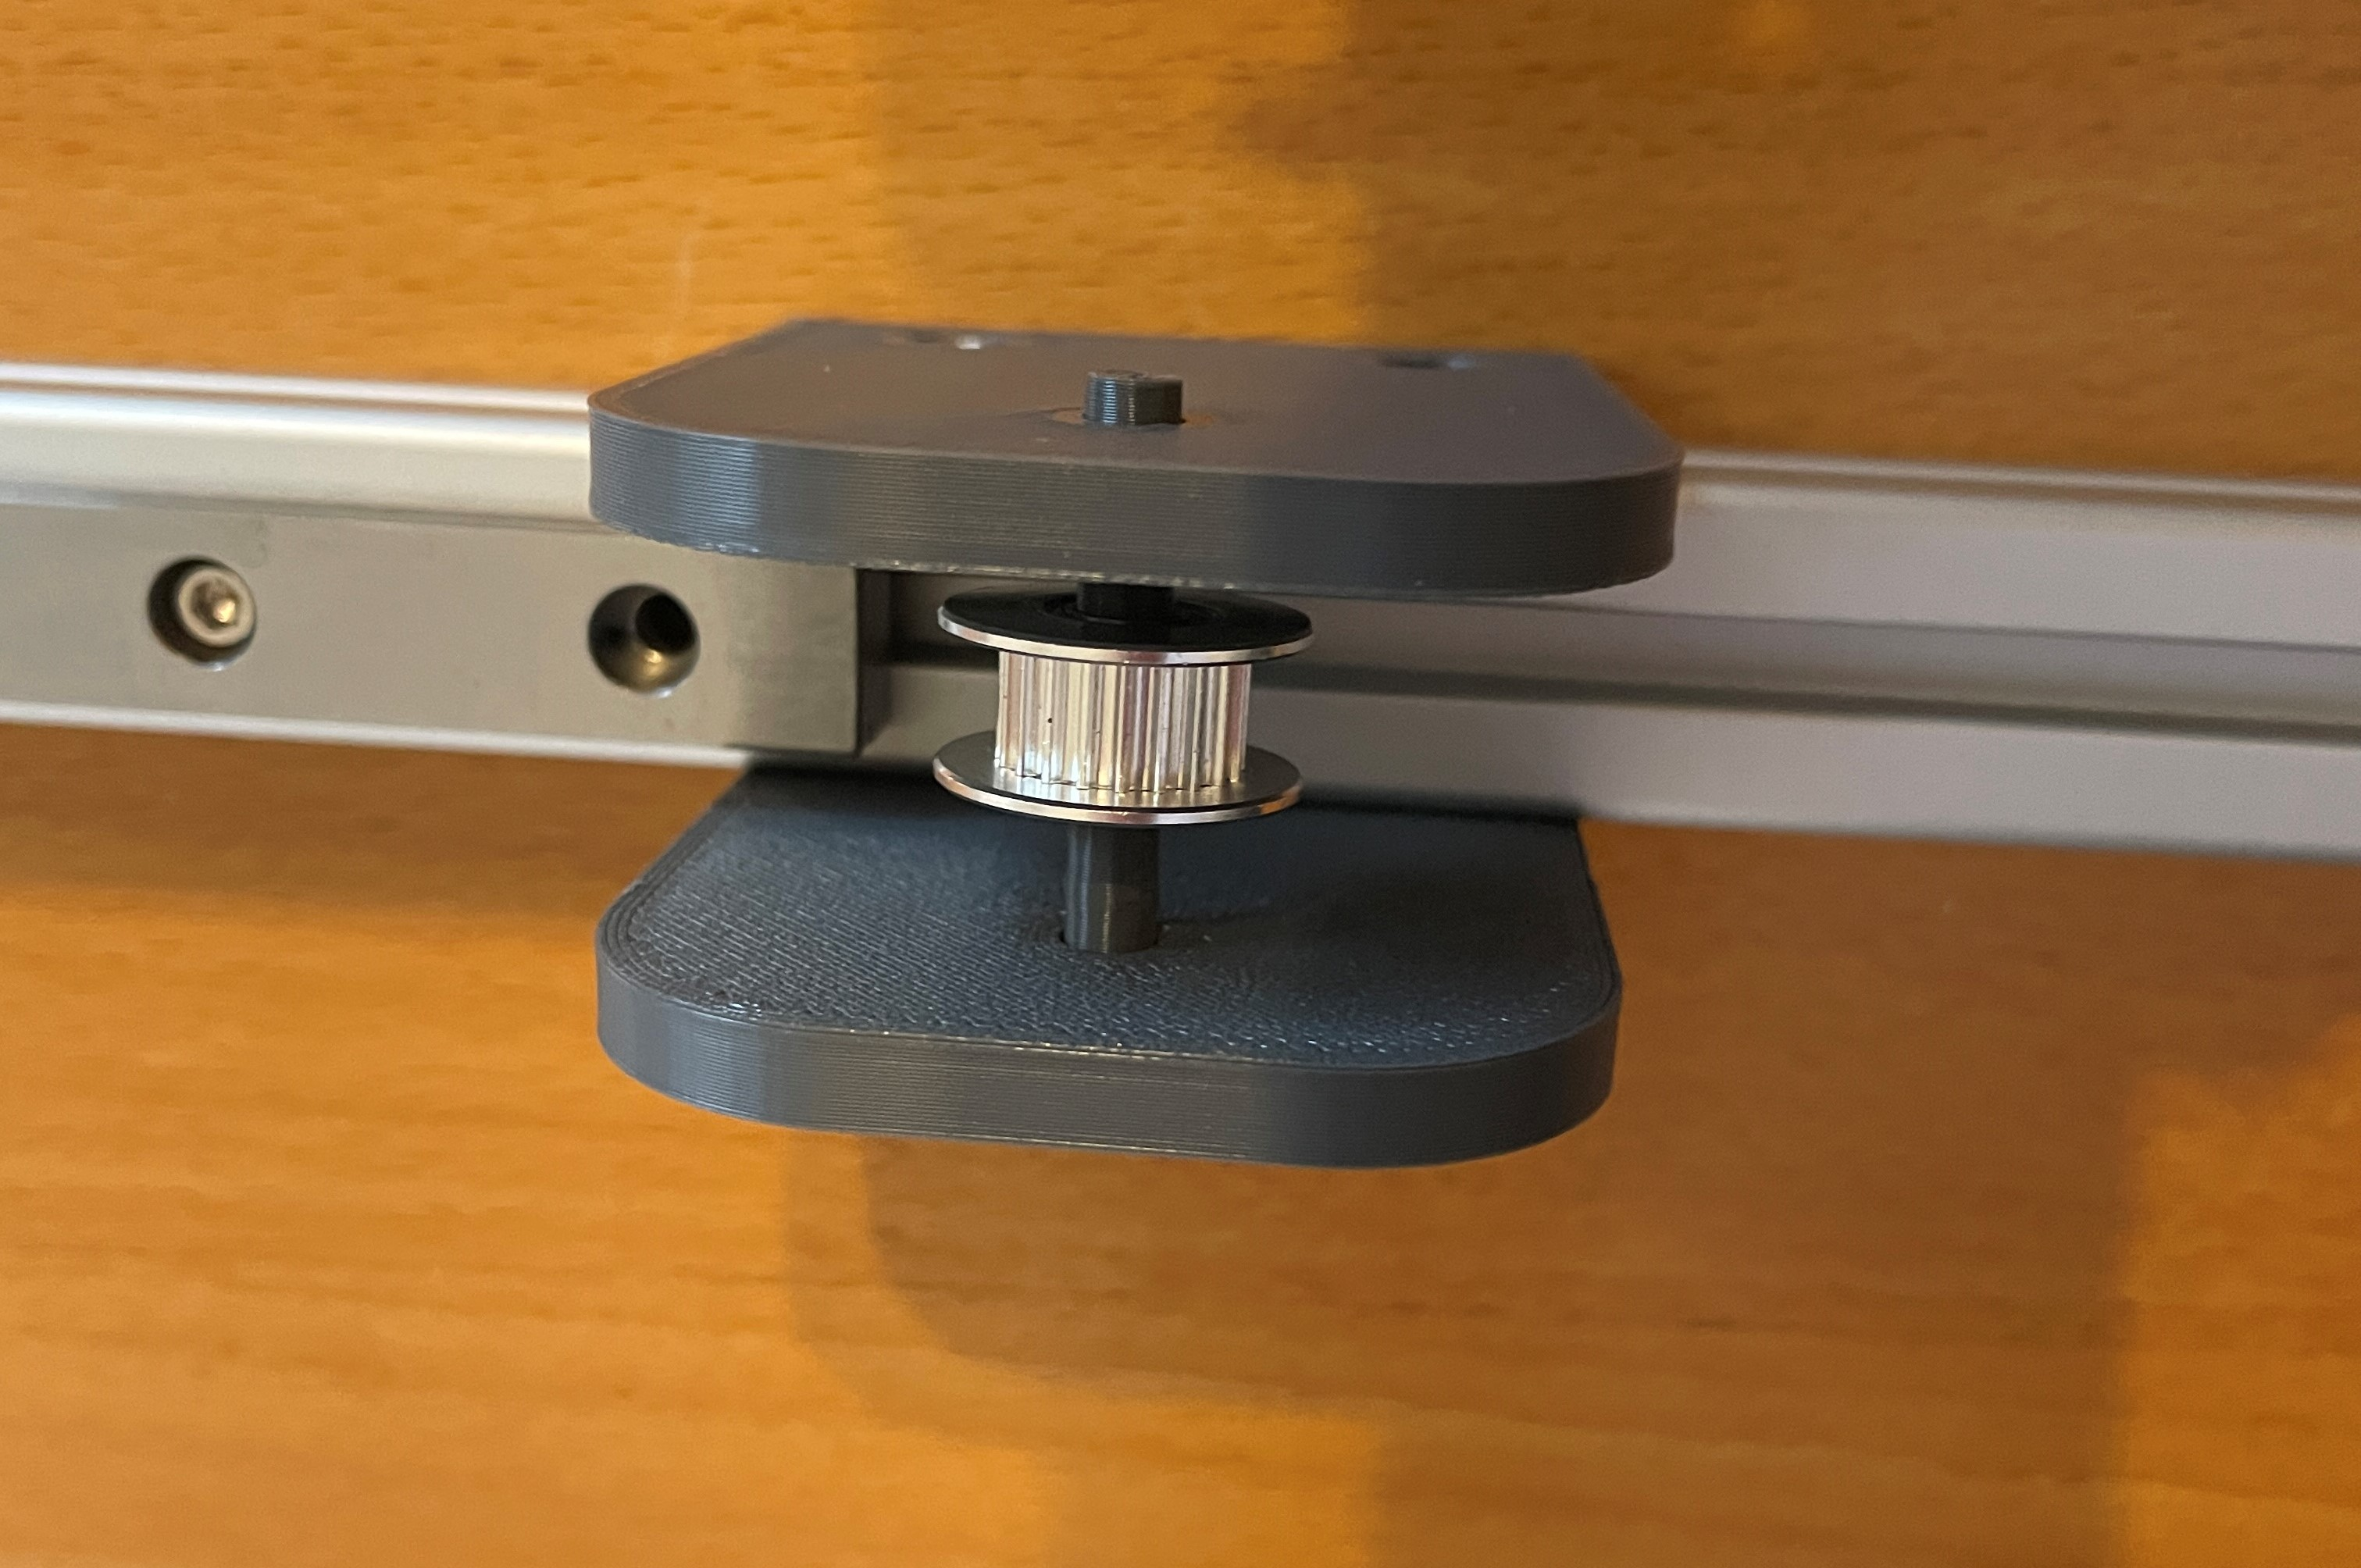
\includegraphics[width=\textwidth]{Images/11Schr.jpg}
		\caption{Elfter Schritt: Montieren der Halter für die Welle} \label{11.S}
	\end{center}
\end{figure}


\section{Zwölfter Schritt: Montieren der Riemenscheibe am Motor}
Montieren Sie die folgenden Bauteile wie in Abbildung \ref{11.S} gezeigt.

\begin{enumerate}
	\item Montieren Sie die Riemenscheibe auf die Welle des Nema 17 Motors und befestigen Sie den mit den Madenschrauben in der Riemenscheibe. 
\end{enumerate}

\begin{figure}[H]
	\begin{center}
		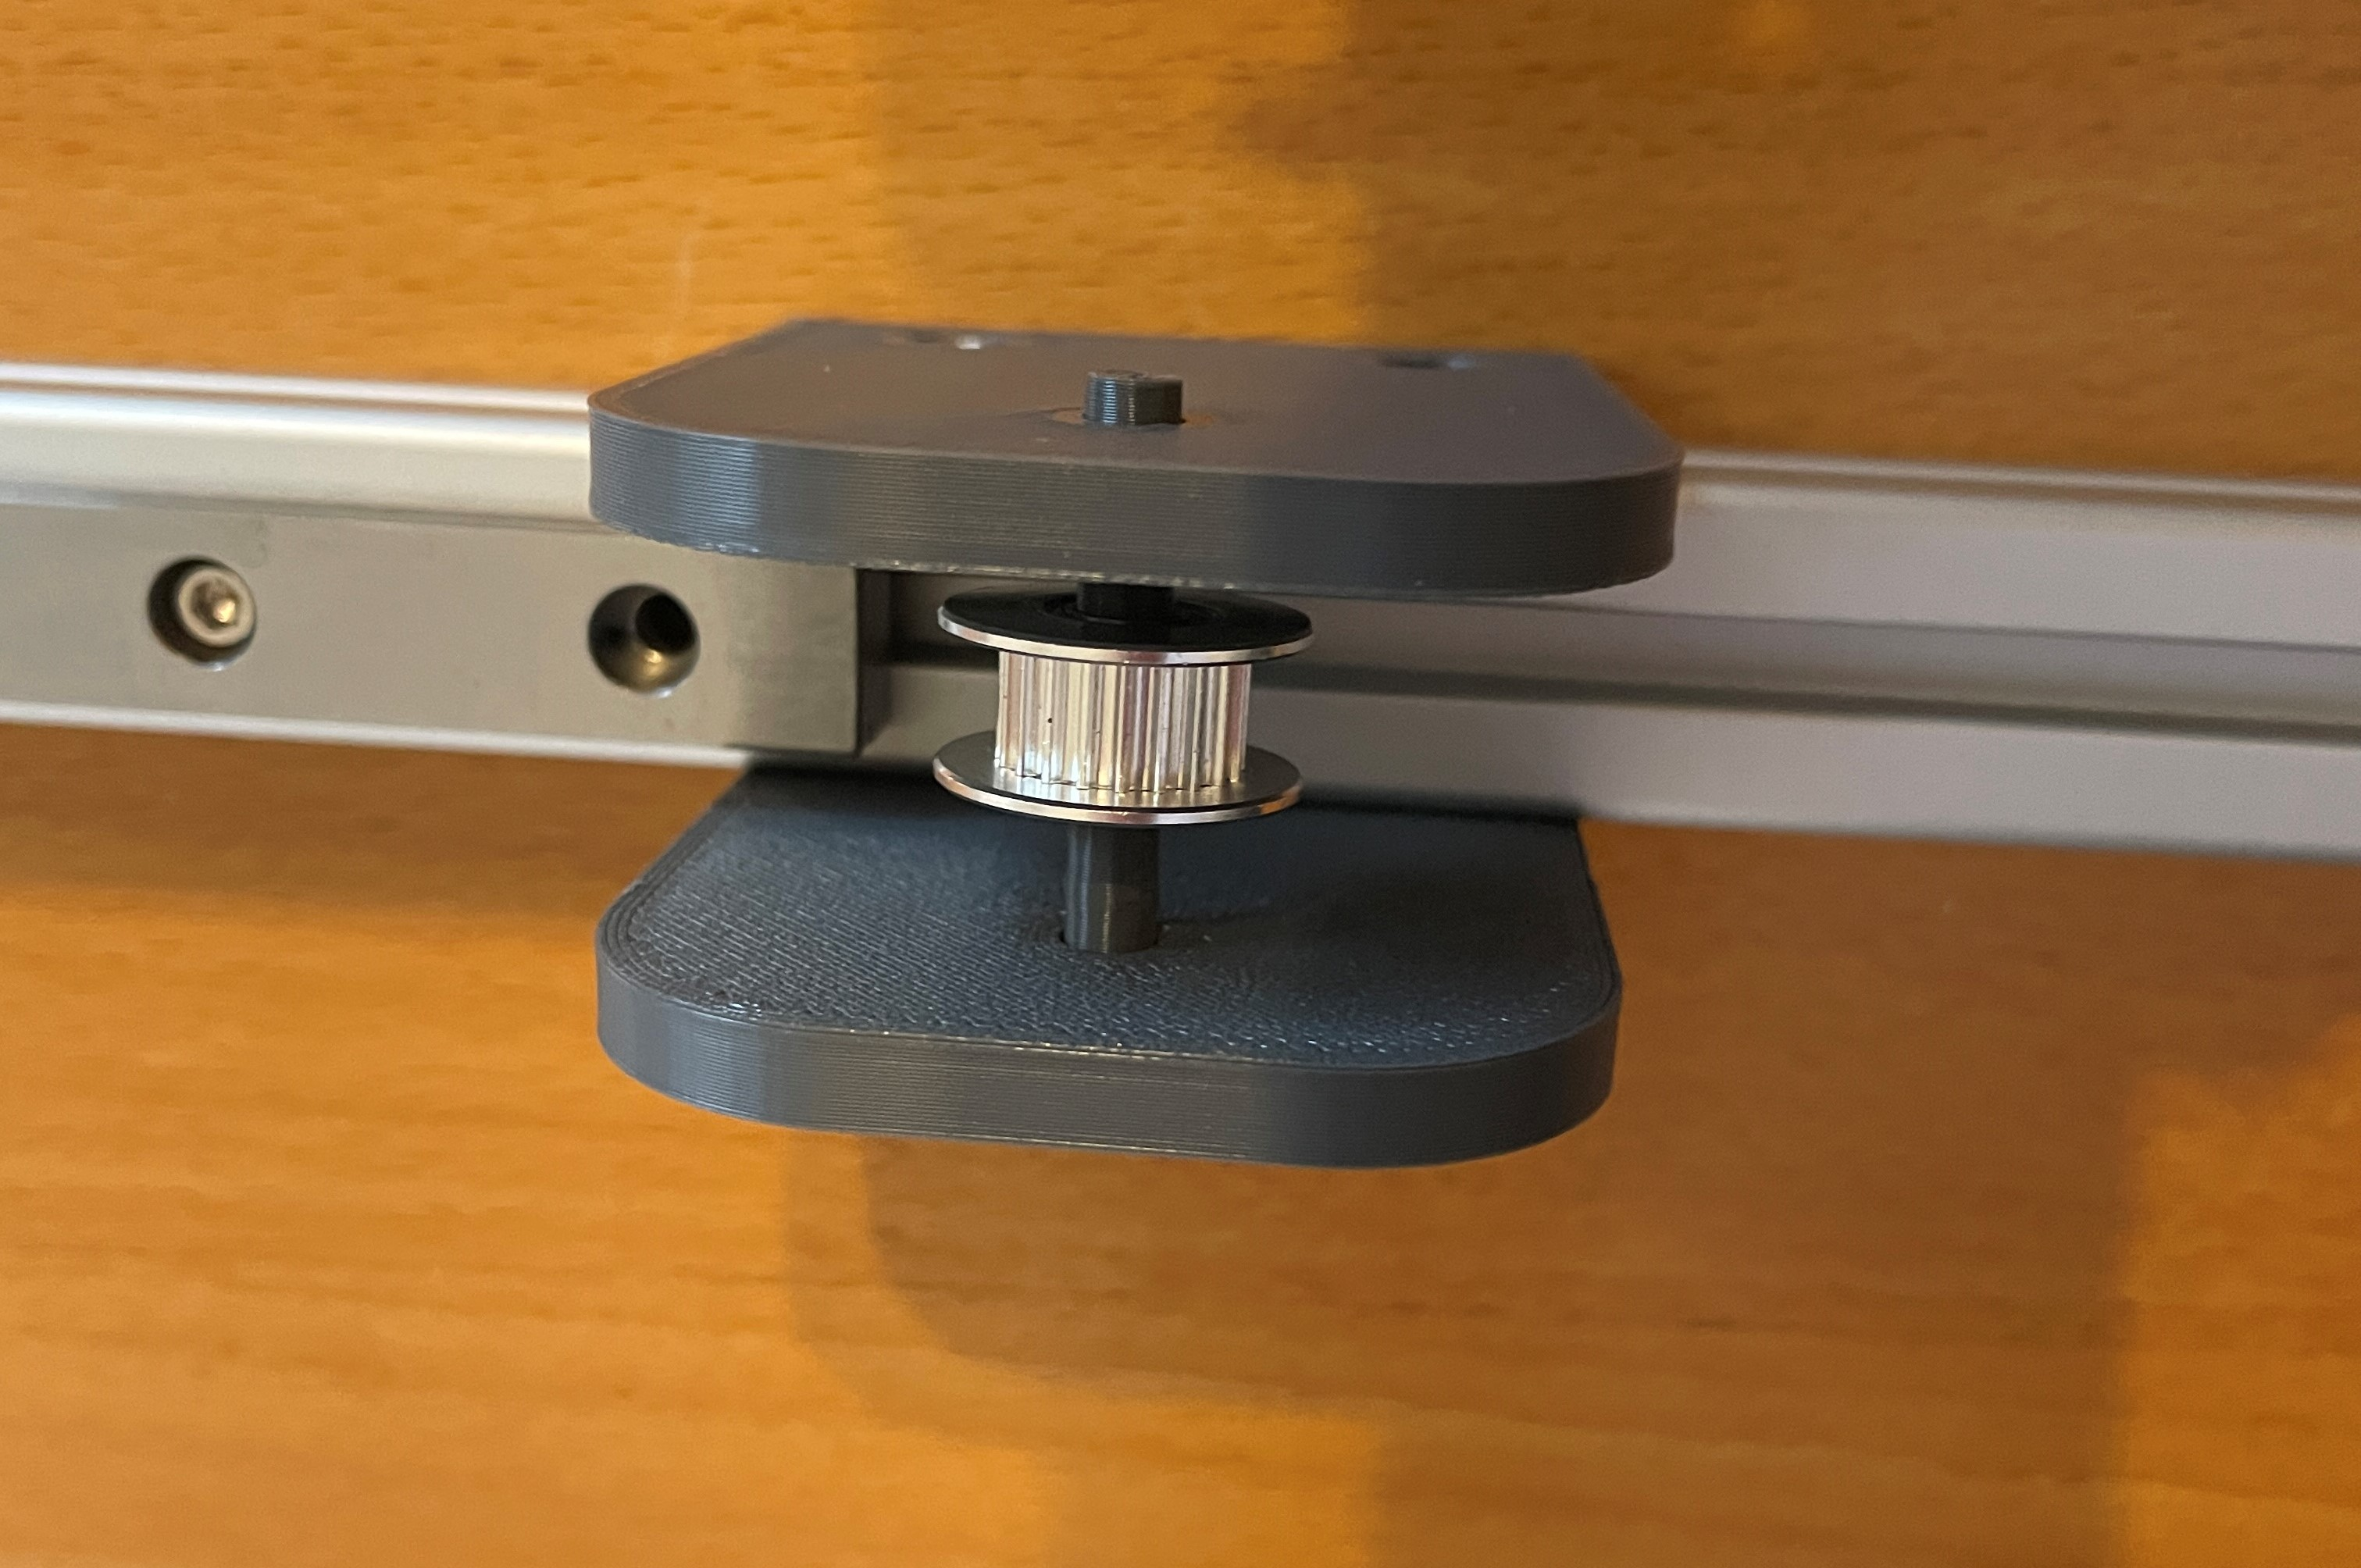
\includegraphics[width=\textwidth]{Images/11Schr.jpg}
		\caption{Zwölfter Schritt: Montieren der Riemenscheibe am Motor} \label{12.S}
	\end{center}
\end{figure}


\section{Dreizehnter Schritt: Montieren des Anzeigers und des Riemens}
Montieren Sie die folgenden Bauteile wie in Abbildung \ref{13.S} gezeigt.

\begin{enumerate}
	\item Montieren Sie den Anzeiger auf den Schlitten der Liniearführung mit 4 $\times$ $ M3 \times 6 \ mm $ Schrauben.
	\item Montieren Sie den Riemen Auf den Anzeiger mit 4 $\times$ $ M3 \times 6 \ mm $ Schrauben.
\end{enumerate}

\begin{figure}[H]
	\begin{center}
		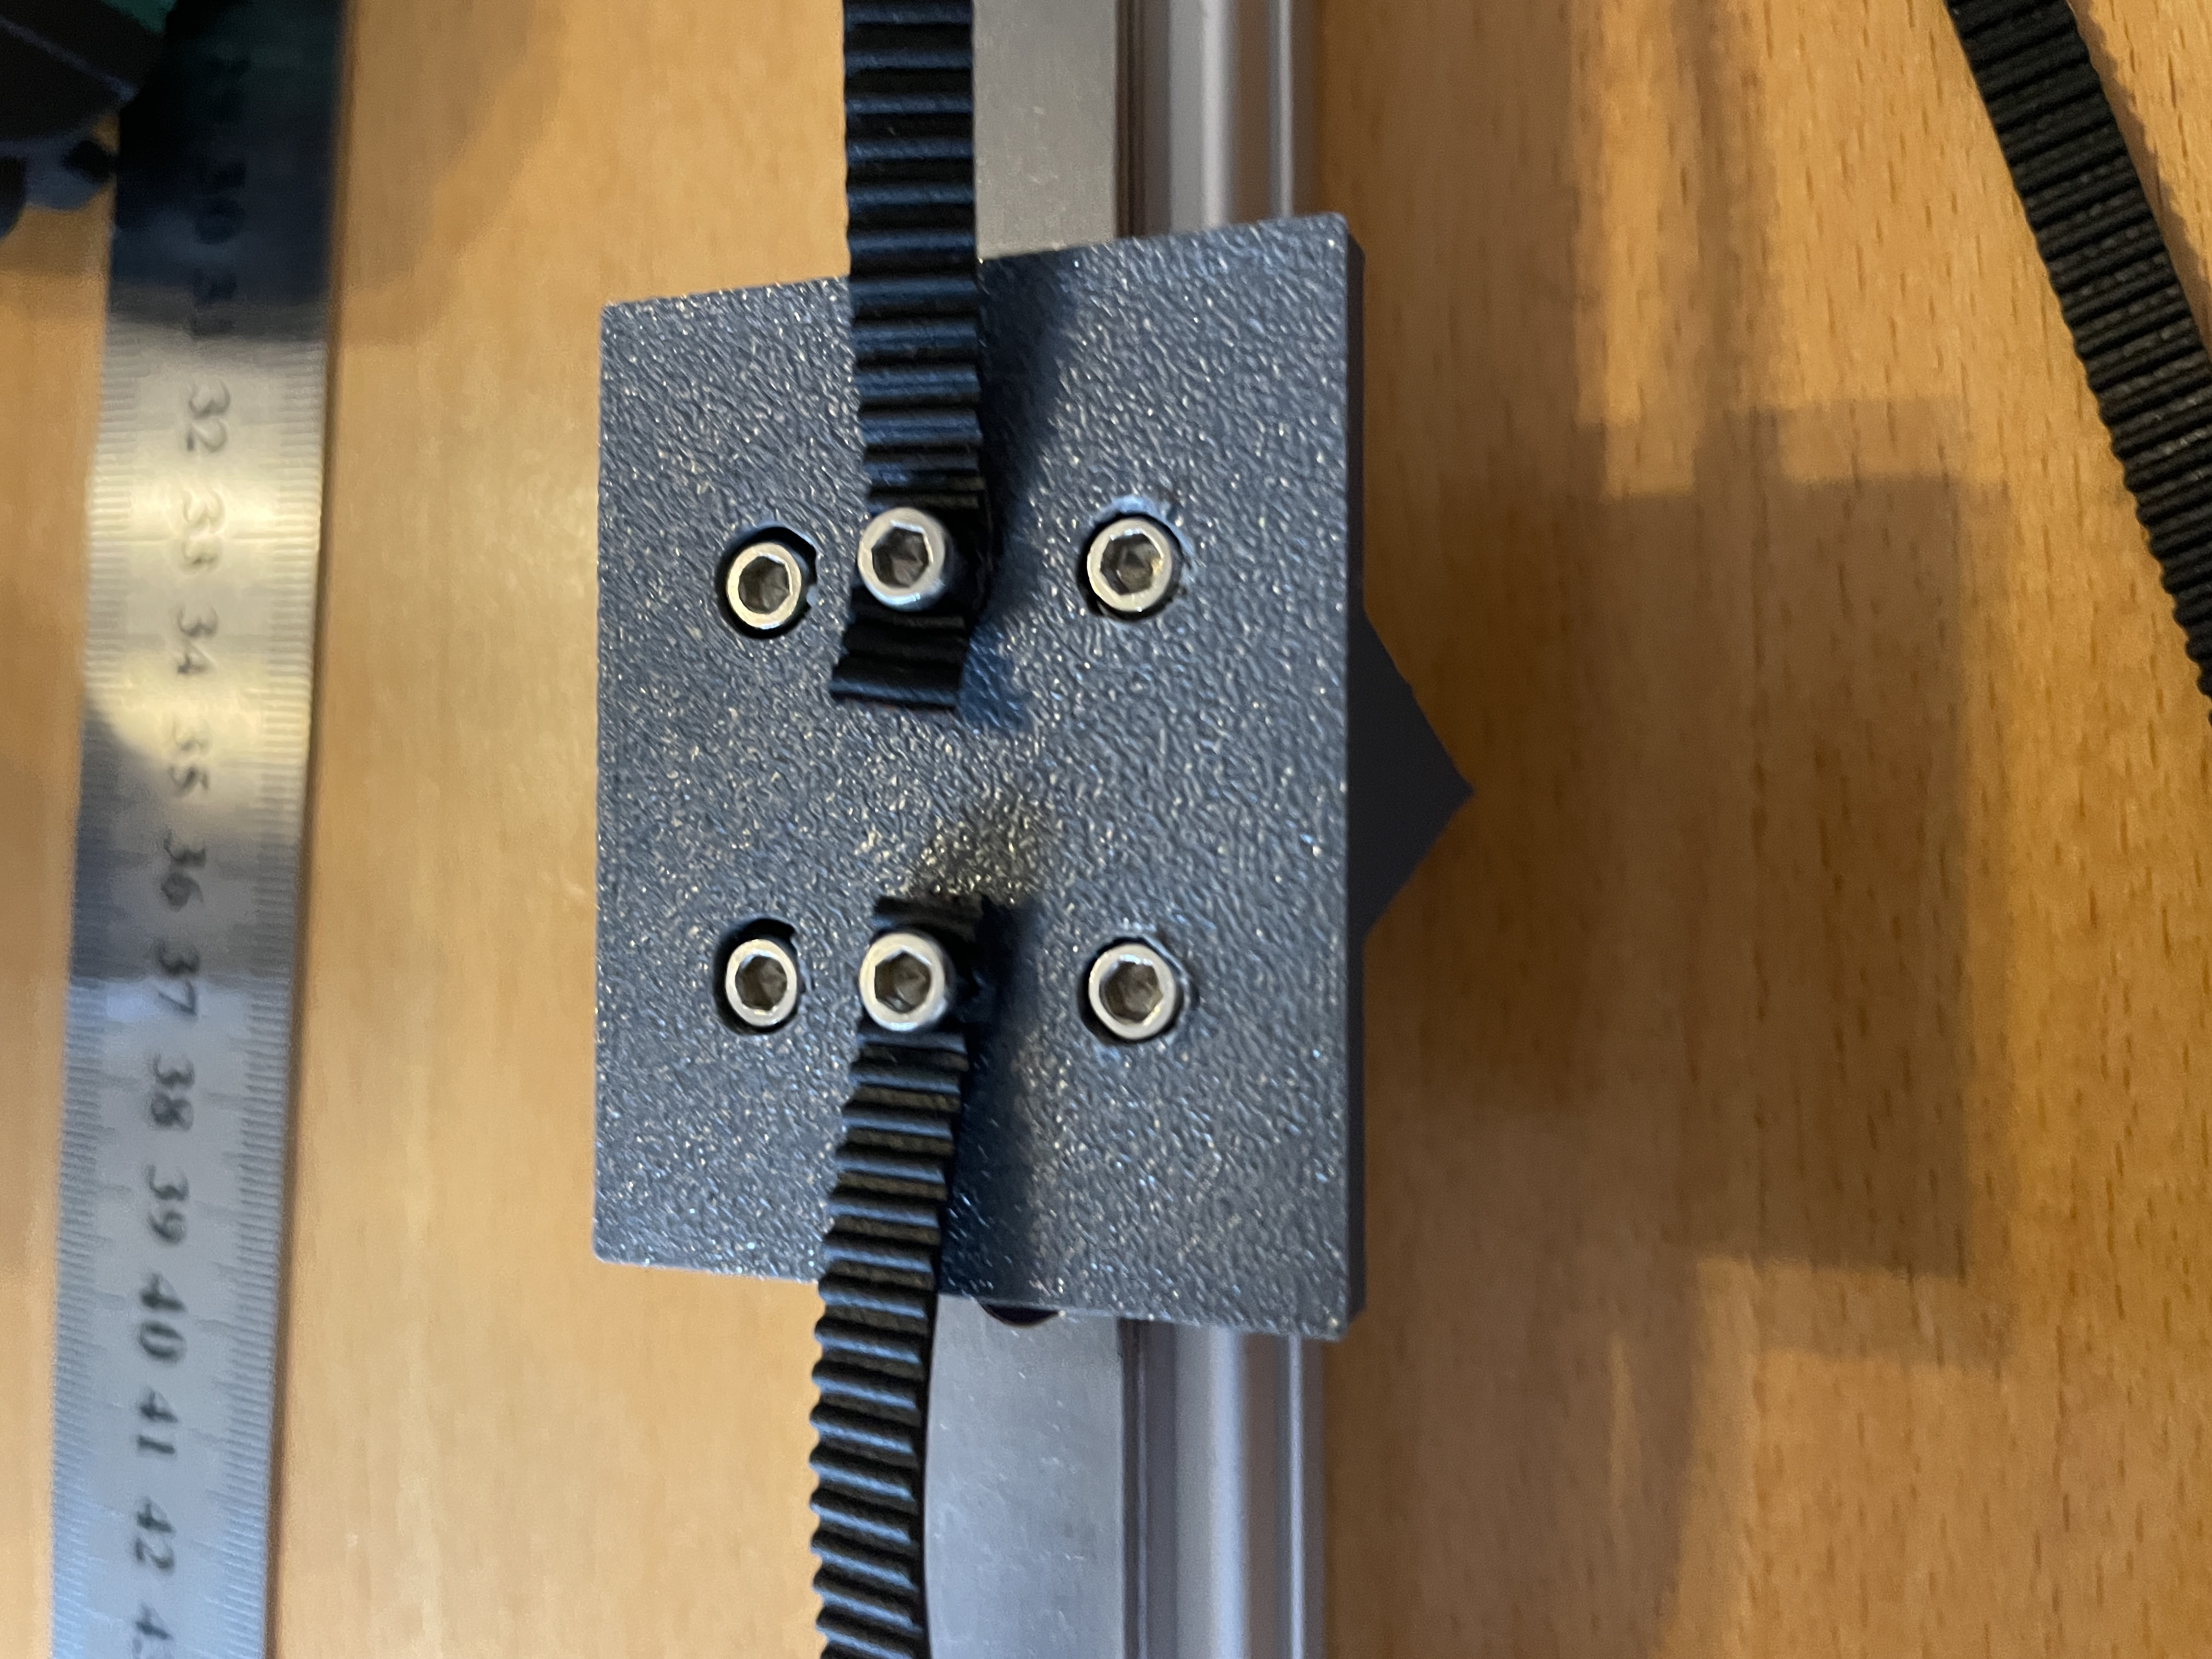
\includegraphics[width=\textwidth]{Images/13Schr.jpg}
		\caption{Zwölfter Schritt: Montieren des Anzeigers und des Riemens} \label{13.S}
	\end{center}
\end{figure}


\section{Vierzehnter Schritt: Montieren des Lineals}

\begin{enumerate}
	\item Montieren Sie das Lineal auf den Schlitten der Liniearführung mit 4 $\times$ $ M3 \times 6 \ mm $ Schrauben mit dem im Schritt 11 eingesetzten 2 $\times$ $ M3 $ Hammermutter.
\end{enumerate}


\section{Abschlussarbeiten}

\begin{enumerate}
	\item Überprüfen Sie alle Verbindungen und Schrauben auf festen Sitz.
	\item Testen Sie Mithilfe des Manuals die Funktionsfähigkeit des Demonstrators. 
\end{enumerate}
